\chapter{Conjuntos de corte y ciclos}

\lettrine[lines=6] {\initfamily \selectfont A} {través} de este capítulo, $G$ será una gráfica conexa con $n$ vértices y $m$ aristas, y cuyo orden es de tal forma que $V(G) = \{u_{1}, \ldots, u_{n}\}$ y $E(G)=\{e_{1}, \ldots, e_{m}\}$. El concepto central de capítulo será el de \textit{subgráfica generadora}, definidas anteriormente. Dicho de forma concreta, abordaremos tres clases especiales de subgráficas de $G$: los \textit{conjuntos de corte}, las \textit{gráficas pares} y los \textit{árboles generadores} (de los que se habló brevemente en el capítulo pasado).

\section{Conjuntos de corte de $G$}

Tomando $X$ y $Y$ dos subconjuntos de vértices, denotaremos por $E[X,Y]$ al conjunto de aristas de $G$ que tienen un extremo en $X$ y otro en $Y$. Si $X = Y$, sólo escribiremos $E[X]$. Si sucediera que $Y$ es el complemento de $X$ respecto a $V$, es decir, que $Y=V \setminus X$, entonces al conjunto $E[X, V \setminus X]$ se le llamará \textit{conjunto de corte de $G$ asociado a $X$} y será escrito como $\partial(X)$. Si $H$ es una subgráfica de $G$ y $X \subseteq V(H)$, entonces $\partial_{H}(X)$ denota al \textit{conjunto de corte relativo a $H$}.

Por comodidad, en lo sucesivo escribiremos $\overline{X}$ en lugar de $V \setminus X$. Así, $\partial(X) = E[X,\overline{X}]$. Es sencillo observar que $\partial(X) = \partial(\overline{X})$ pues, por definición, $E[X,\overline{X}] = E[\overline{X},X]$. En particular, $\partial(V)=\partial(\emptyset) = \emptyset$. También puede deducirse que, para cada  $v \in V$, $\partial(\{v\})$ es el conjunto de todas las aristas que inciden en $v$, excluyendo sus lazos.  A veces escribimos $\partial(v)$ en lugar de $\partial(\{v\})$.

$\partial(X)$ también denota a la subgráfica generadora de $G$ cuyo conjunto de aristas es, precisamente, el corte asociado a $X$; y tal subgráfica también se llama \textit{conjunto de corte}. Vale la pena aclarar que, aunque lo anterior es un abuso de notación, trabajaremos con $\partial(X)$ tanto como conjunto de aristas y como subgráfica generadora de $G$.

\begin{ejem} \label{ejem:cjtosdecorte}
Consideremos la gráfica del inciso $(b)$ de la figura \ref{fig:cjtosdecorte}. En $(b)$ represantamos el conjunto de aristas $E[A,B] = \{b,c,f,g\}$, con $A=\{u_{1}, u_{2}, u_{3}\}$ y $B=\{u_{3},u_{4}\}$. En $(c)$ tomamos $X =\{u_{1},u_{5}\}$, y verificamos que $\partial(X) = \{a,f,g,d\}$.
\begin{figure}[H]
    \centering
    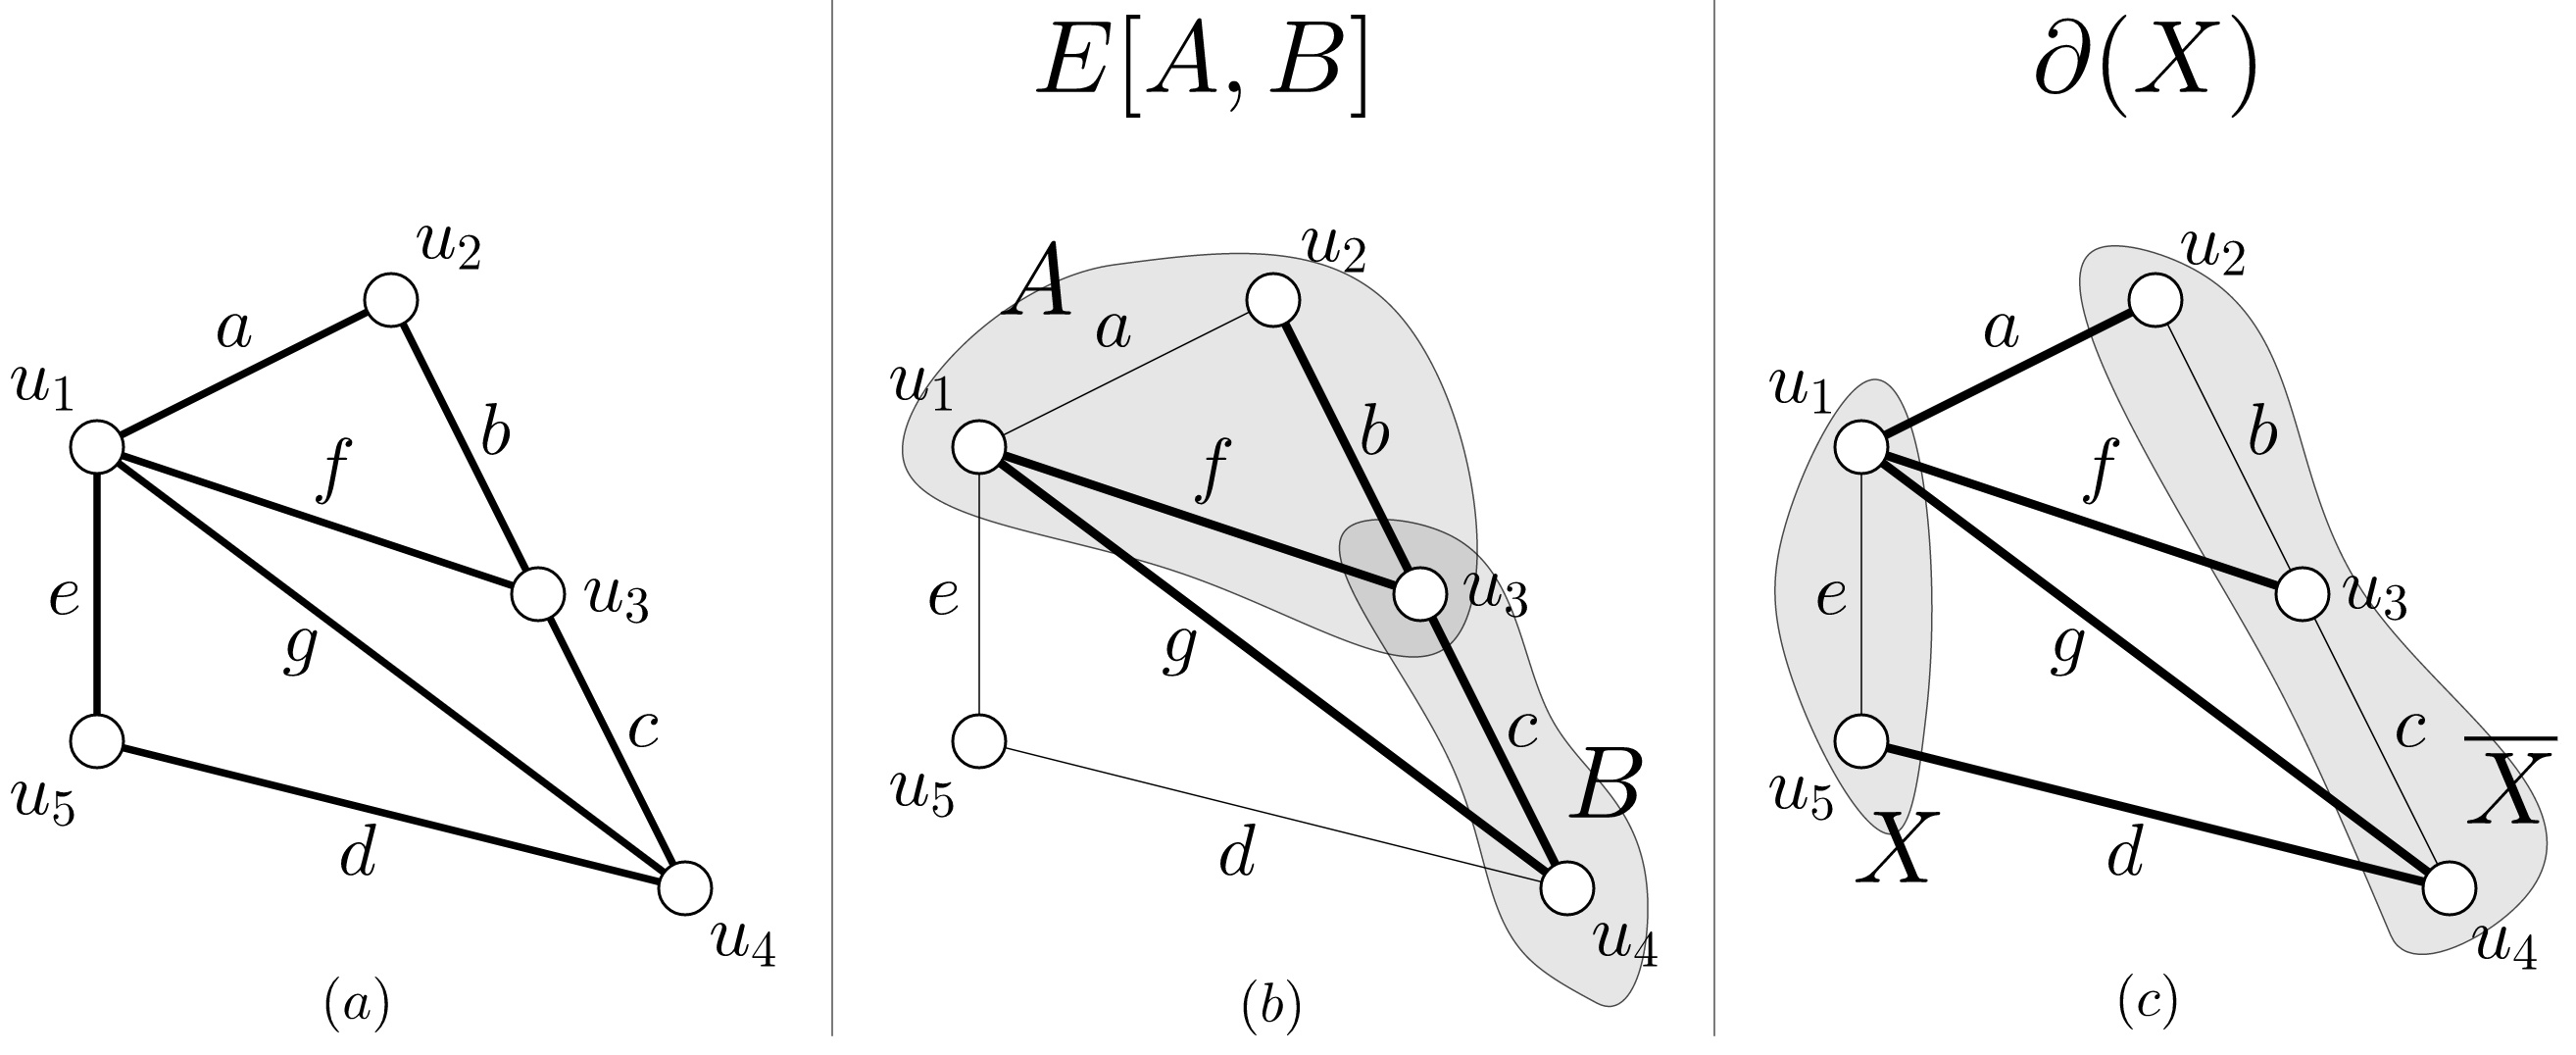
\includegraphics[scale=0.2]{img/imgchapter2/cjtosdecorte.jpg}
    \caption{}
    \label{fig:cjtosdecorte}
\end{figure}

\hfill $\blacklozenge$
\end{ejem}
Observe que nuestra nueva notación ayuda reformular la definición de \textit{gráfica conexa} que dimos en el capítulo anterior (y que utilizaremos en los teoremas siguientes) una gráfica $G$ será conexa si y sólo si $\partial(X) \neq \emptyset$, para todo $X \subsetneqq V(G)$. 

De hecho, respecto a la conexidad, podemos darnos cuenta que si removemos de $G$ las aristas que pertenecen a $\partial(X)$, entonces la subgráfica $G\setminus \partial(X)$ es inconexa, justificando así el nombre ``conjunto de corte'' que le dimos a $\partial(X)$, pues éstos desconectan a $G$. Si tomamos en cuenta la gráfica del ejemplo \ref{ejem:cjtosdecorte} y hacemos $X=\{u_{1},u_{4}\}$, vemos que $G\setminus \partial(X)$ tiene tres componentes conexas.

\begin{figure}[H]
     \centering
     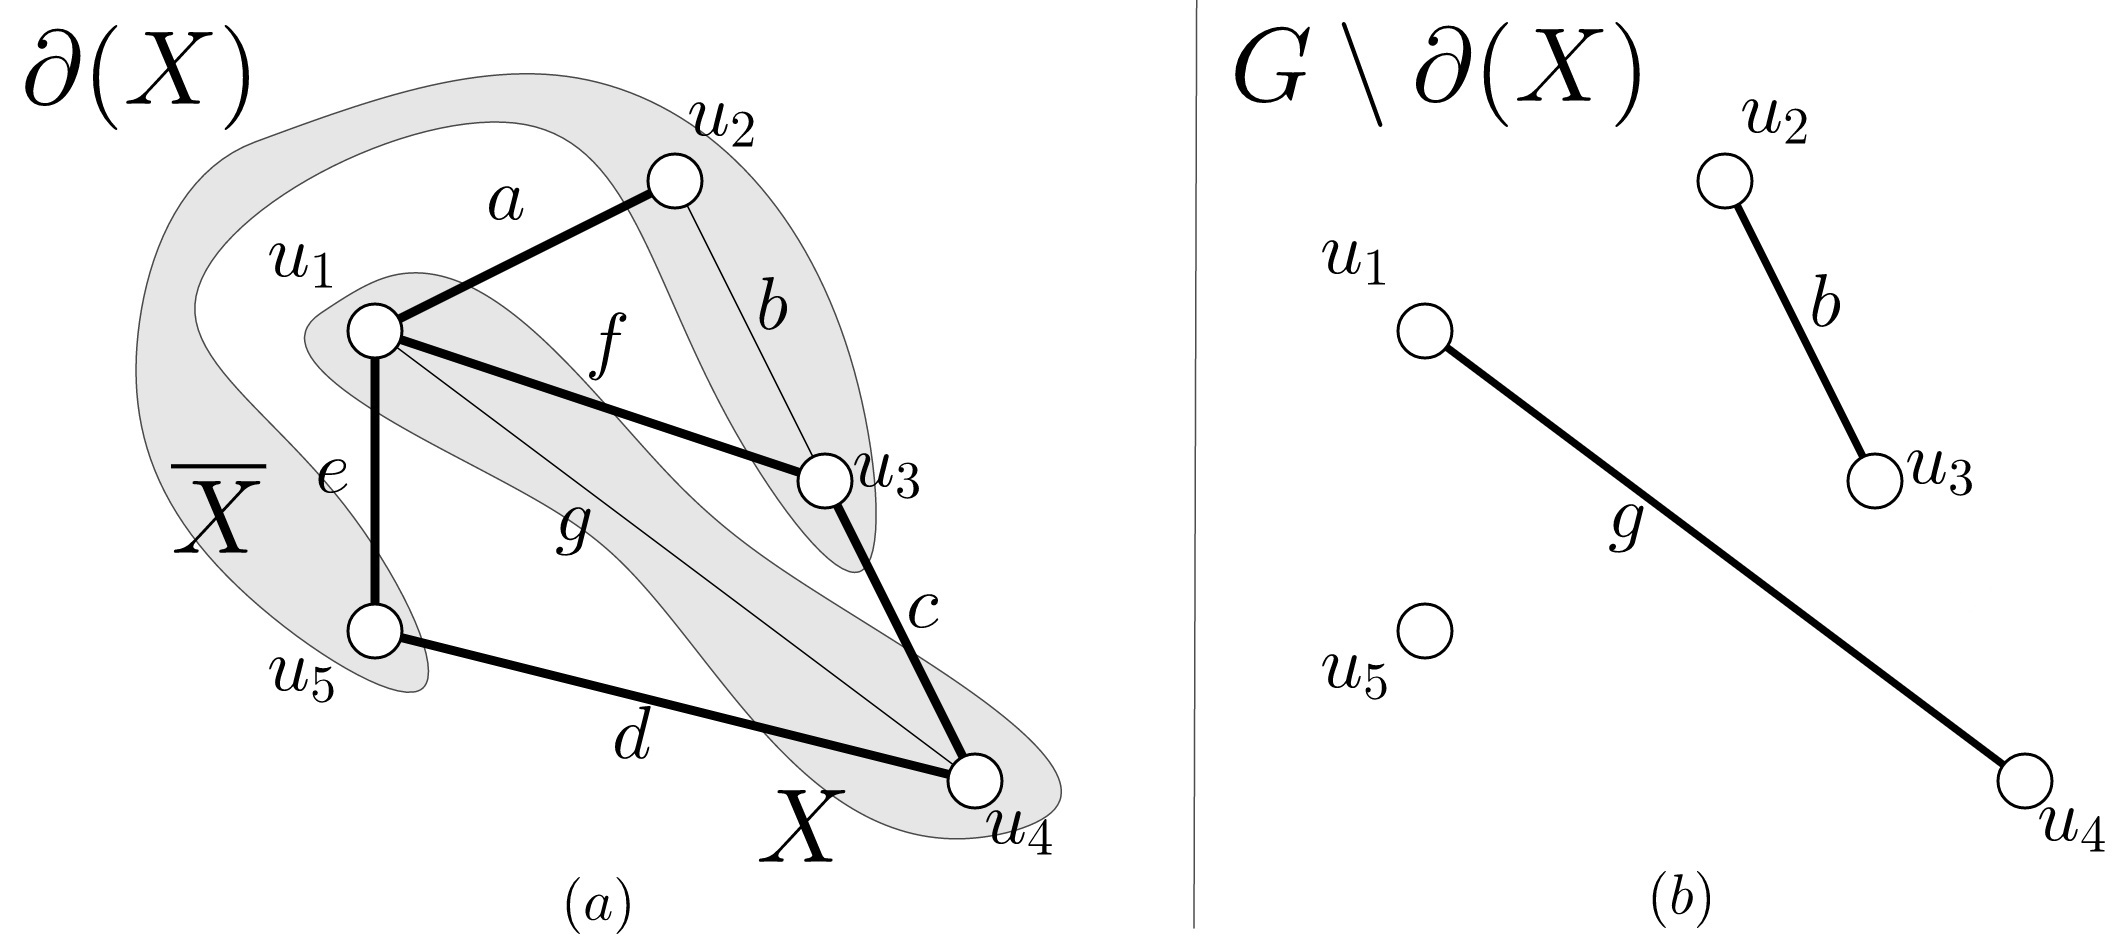
\includegraphics[scale=0.2]{img/imgchapter2/cortescompconexas.jpg}
     \caption{}
     \label{fig:cortescompconexas}
\end{figure}

Analizaremos ahora qué propiedades tienen los conjuntos de corte
\begin{teo}\label{teo:diferenciasimetricacortes}
Sea $G$ una gráfica y sean $X$ y $Y$ subconjuntos de $V$. Entonces $$\partial(X) \triangle \partial(Y) = \partial(X \triangle Y).$$
\end{teo}

\begin{proof}
Recordemos que $X \triangle Y = (X \cup Y)\setminus(X \cap Y) = (X \cup Y) \cap (\overline{X \cap Y}) = (X \cup Y) \cap (\overline{X} \cup \overline{Y})$. Y de esta última igualdad, tenemos que 
\begin{equation} \label{eq1}
    X \triangle Y = (\overline{X}\cap Y) \cup (X \cap \overline{Y}).
\end{equation}

Por otro lado, $\overline{X \triangle Y}=\overline{(X \cup Y) \cap (\overline{X \cap Y})}= \overline{X \cup Y} \cup (X \cap Y)$. Así, llegamos a que
\begin{equation} \label{eq2}
   \overline{X \triangle Y} = (X \cap Y) \cup (\overline{X} \cap \overline{Y}).
\end{equation}

Como $V(G)=(X \triangle Y) \cup (\overline{X \triangle Y})$, de las igualdades \ref{eq1} y \ref{eq2} se sigue que 
\begin{equation} \label{eq3}
    V(G) = (X \cap Y) \cup (\overline{X} \cap \overline{Y}) \cup (\overline{X} \cap Y) \cup (X \cap \overline{Y}).
\end{equation}

La igualdad \ref{eq3} sugiere que los cuatro conjuntos involucrados en su lado derecho forman una partición de $V(G)$ (pues son ajenos dos a dos). Tomando en cuenta las definiciones de $\partial(X), \partial(Y)$ y  $\partial(X \triangle Y)$, en la figura \ref{fig:cortessim} se representa el comportamiento de éstos con respecto a la partición del conjunto de vértices de $G$. Aquí, una línea remarcada es un conjunto de aristas cuyos extremos están en algún subconjunto de vértices de la partición anterior.

Si, por simplicidad, hacemos 
\begin{align*}
    J &= \big ( E[X \cap Y, \overline{X} \cap Y] \big ) \bigcup \big(E[X \cap \overline{Y}, \overline{X} \cap \overline{Y}]\big), \\
    K &= \big(E[X \cap Y, X \cap \overline{Y}]\big) \bigcup \big(E[\overline{X} \cap Y, \overline{X} \cap \overline{Y}]\big), \\
    D &= \big(E[X \cap Y, \overline{X} \cap \overline{Y}]) \bigcup (E[X \cap \overline{Y}, \overline{X} \cap Y]\big),
\end{align*}
entonces es fácil darse cuenta (gracias a la figura \ref{fig:cortessim}) que $\partial(X)= J \cup D$, $ \partial(Y)= K \cup D$ y $\partial(X \triangle Y)= J \cup K.$

\begin{figure}[H]
    \centering
    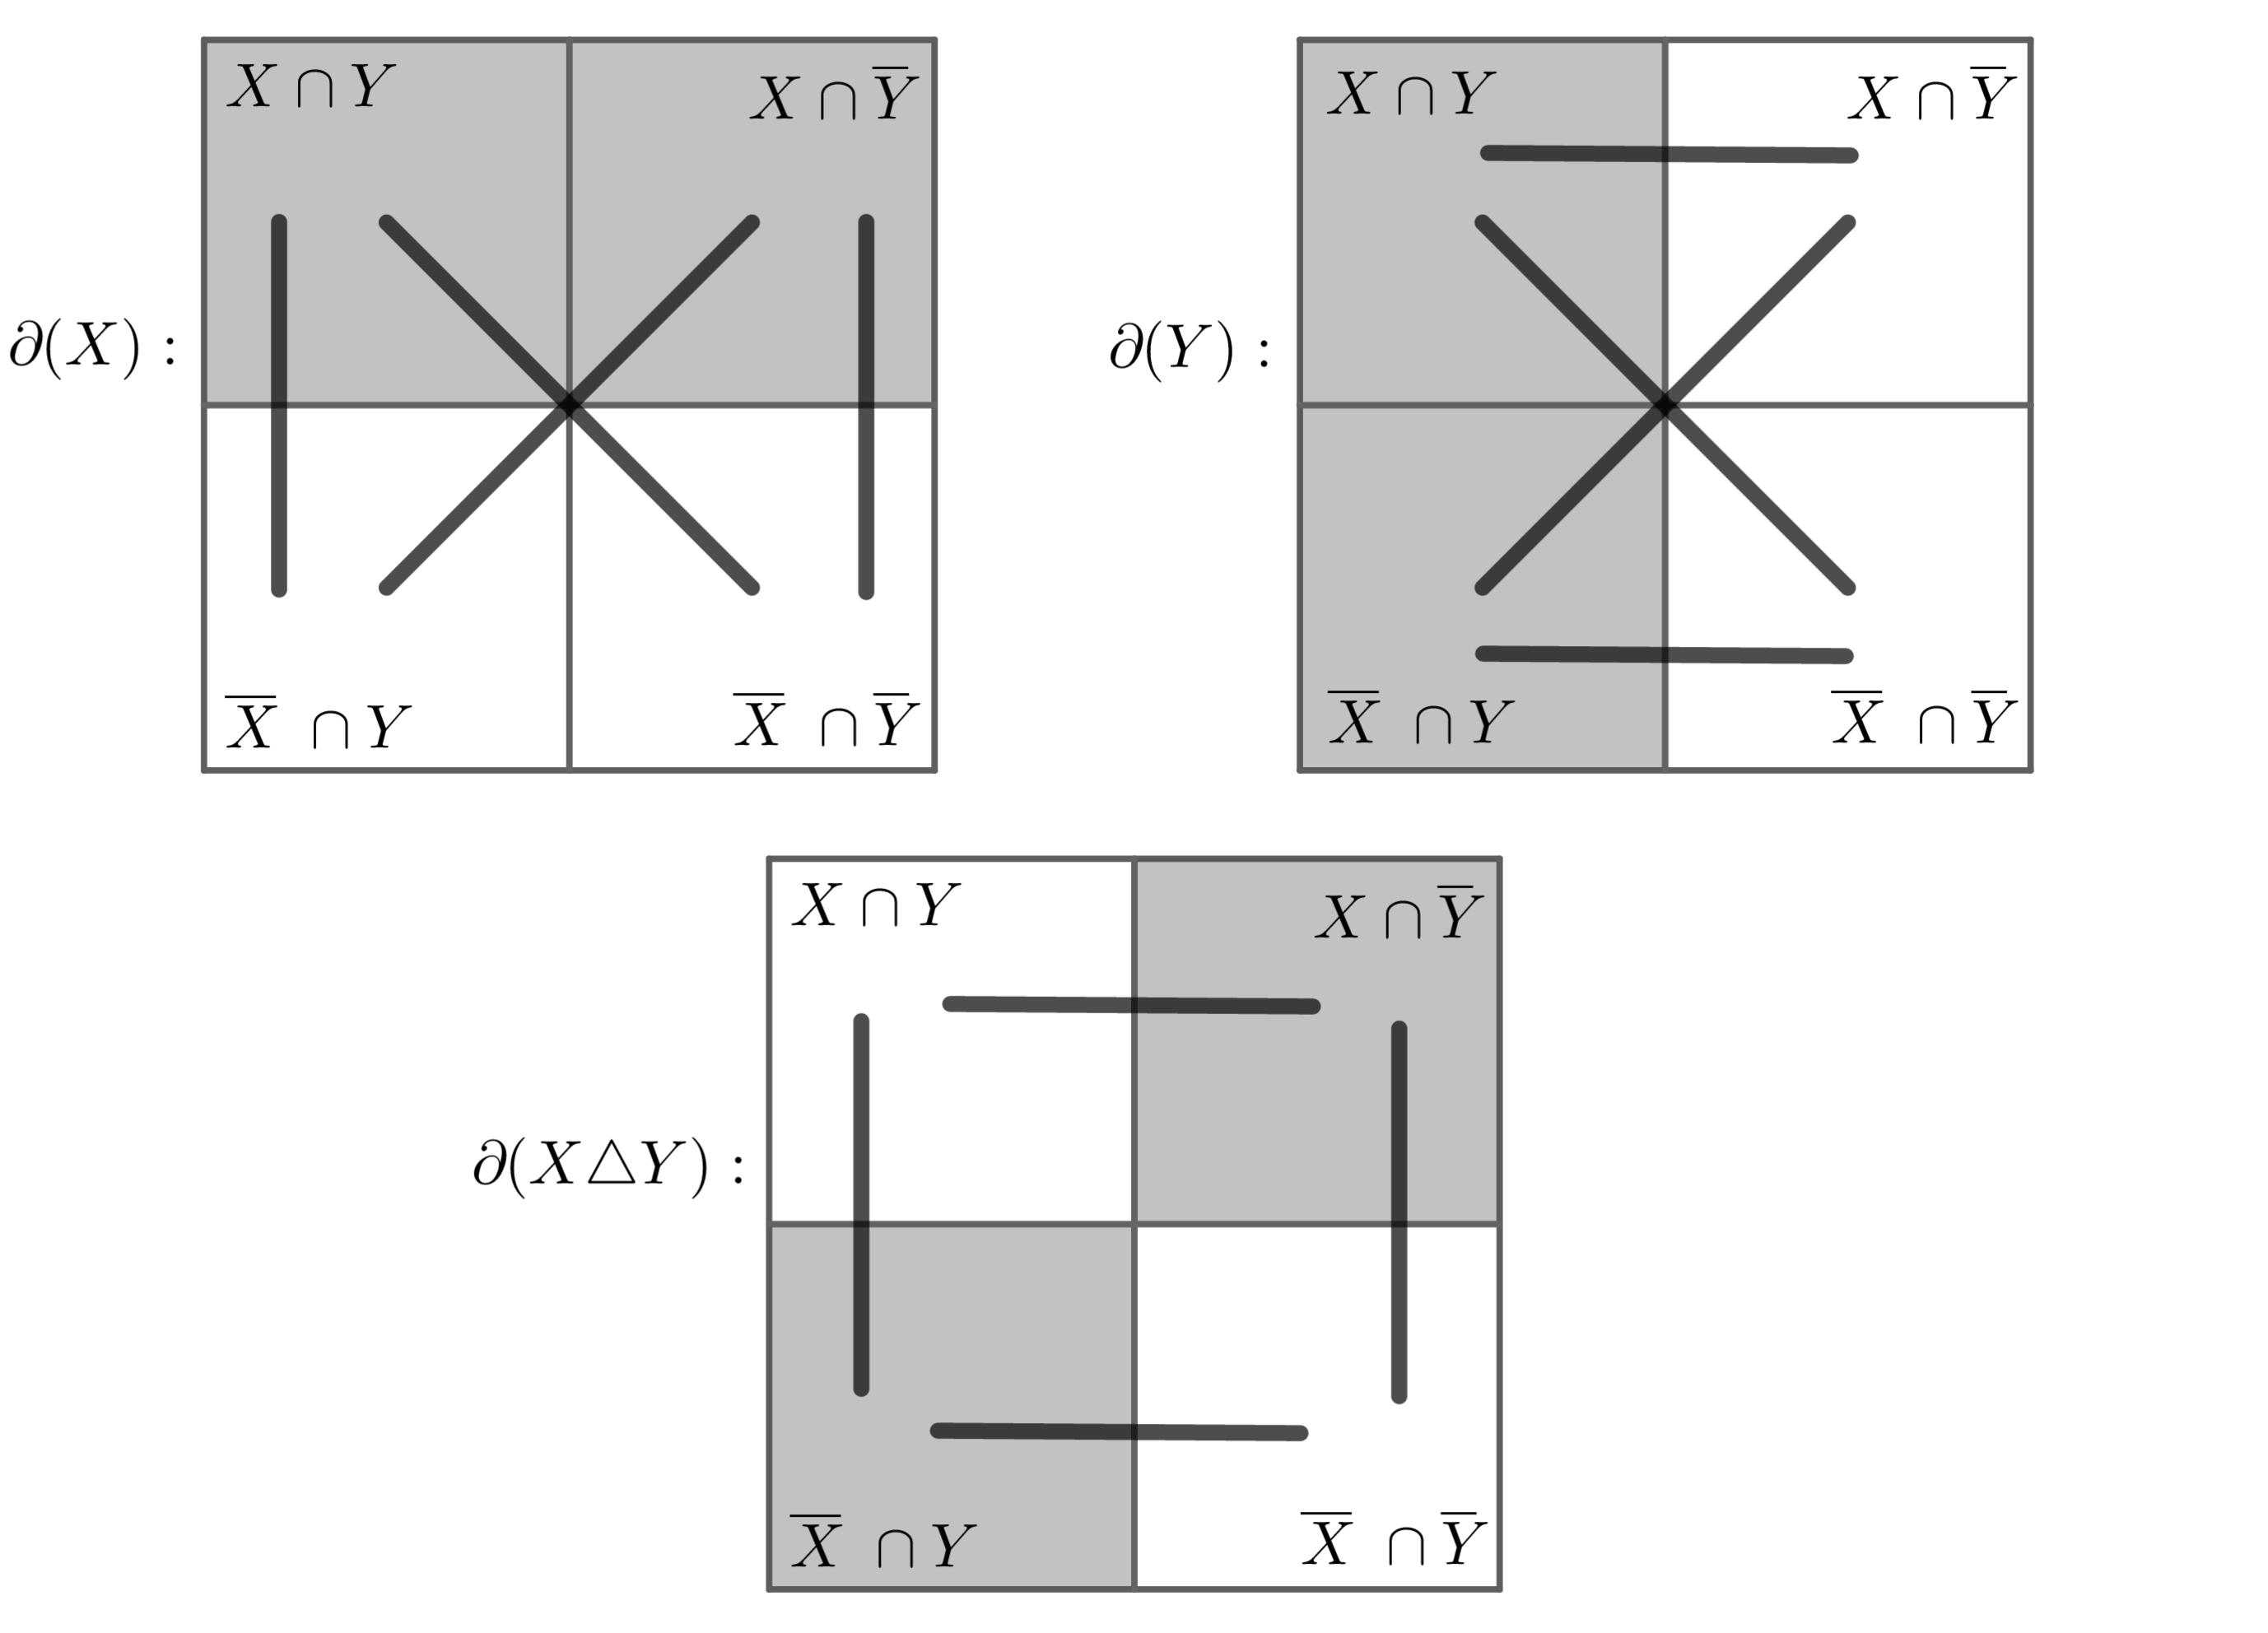
\includegraphics[width=0.75\textwidth]{img/imgchapter2/cortessim.jpg}
    \caption{Diferencia simétrica de dos conjuntos de corte}
    \label{fig:cortessim}
\end{figure}

Luego, observemos que $\partial(X) \triangle \partial(Y) = (J \cup D) \triangle (K \cup D) = (J \cup D) \triangle (K \cup D) =  \big((J \cup D) \setminus (K \cup D)\big) \cup  \big((K \cup D) \setminus (J \cup D)\big) = (J \setminus K) \cup (K \setminus J)$, pues los conjuntos de aristas que tomamos son ajenos mutuamente. Por eso mismo, $(J \setminus K) \cup (K \setminus J) = J \cup K = \partial(X \triangle Y).$

En consecuencia, $\partial(X) \triangle \partial(Y) = \partial(X \triangle Y).$


\end{proof}


\begin{ejem}
\begin{figure}[H]
    \centering
    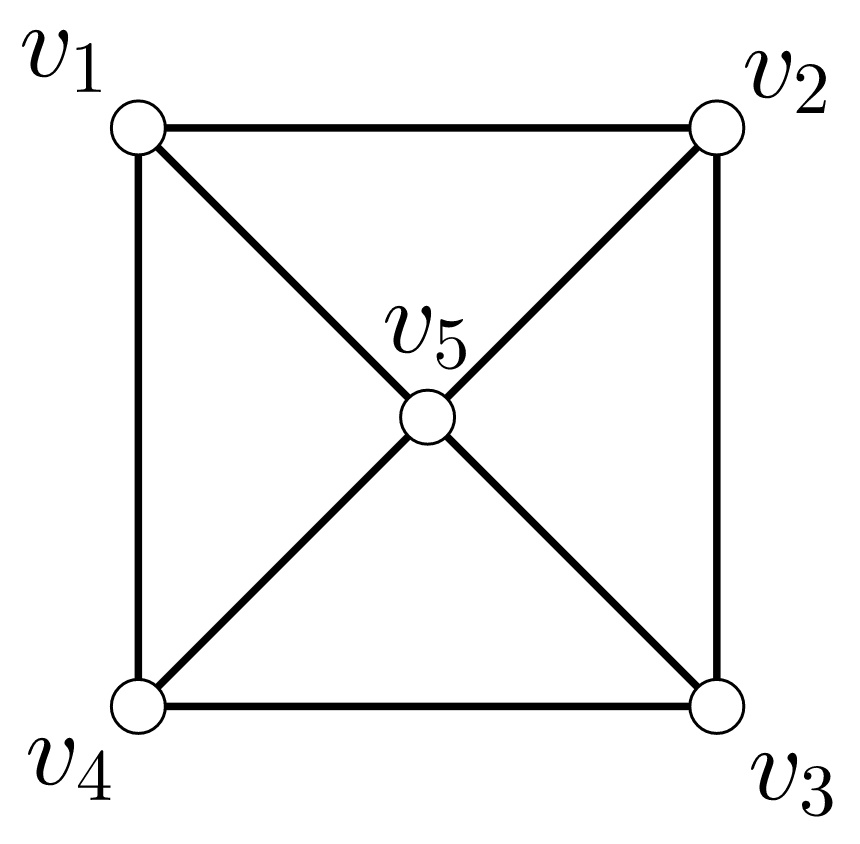
\includegraphics[scale=0.2]{img/imgchapter2/wheel.jpg}
    \caption{}
    \label{fig:wheel}
\end{figure}

Consideremos la gráfica \textit{rueda} $W_{4}$ de la figura \ref{fig:wheel}.
A continuación se muestra sus conjuntos de corte. Hemos resaltado los vértices respecto a los cuales se construye el corte en cuestión y las aristas de éste también se han remarcado. 

\begin{figure}[H]
    \centering
    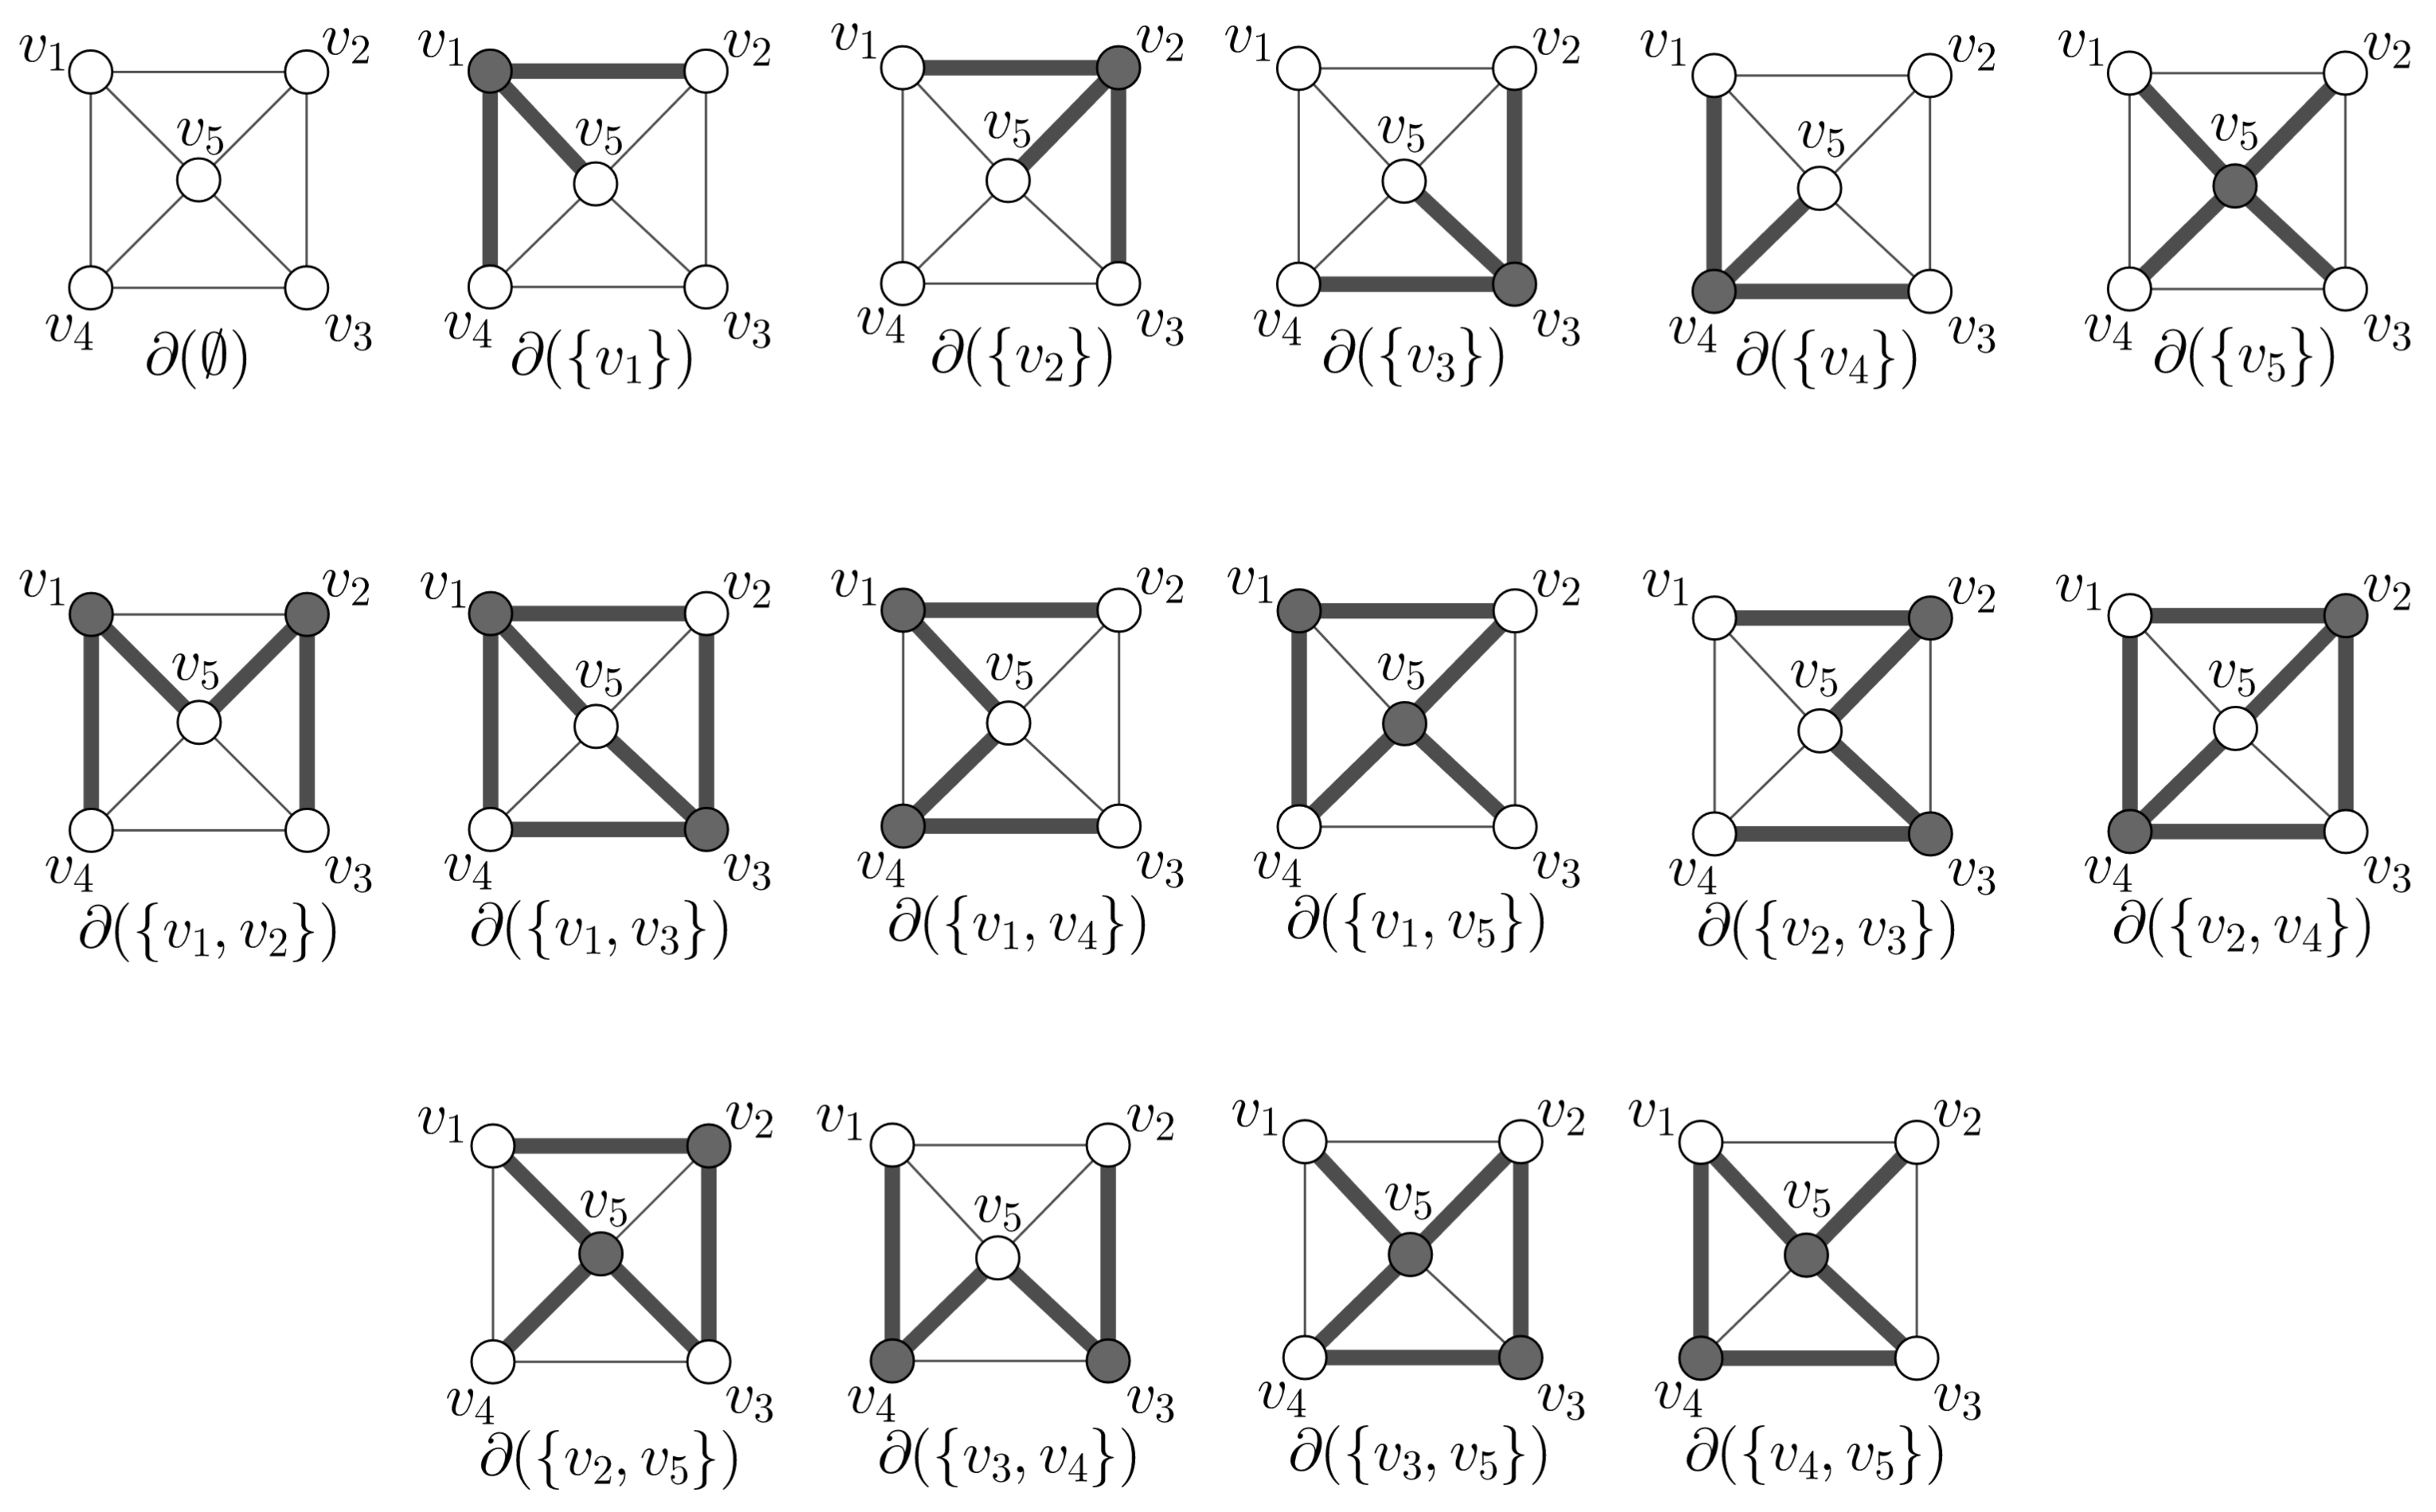
\includegraphics[width=1\textwidth]{img/imgchapter2/espaciocortes.jpg}
    \caption{Cortes de $W_{4}$}
    \label{fig:cortesw4}
\end{figure}

\hfill $\blacklozenge$
\end{ejem}

\subsection{Conjuntos de corte minimales}

Llamamos \textit{conjunto de corte minimal} \footnote{Algunos autores lo llaman \textit{bond}, en inglés.} de $G$ a un conjunto de corte no vacío con la propiedad de que ninguno de sus subconjuntos propios, no vacíos, es otro conjunto de corte. 

Una caracterización fundamental de este tipo de conjuntos de corte nos la da el teorema siguiente. Recordemos que $G[X]$ es la gráfica inducida por el conjunto de vértices $X$.

\begin{teo} \label{teo:caracterizacionbond}
Sean $G$ una gráfica conexa y $X$ un subconjunto de vértices de $G$, de tal manera que $\partial(X) \neq \emptyset$. Entonces $\partial(X)$ es un conjunto de corte minimal si y sólo si $G[X]$ y $G[\bar{X}]$ son conexas. 
\end{teo}

\begin{proof} Asumimos que $G$ es conexa y que $X \subseteq V(G)$.

Probaremos la necesidad por contrapuesta. Supóngase primero que $G[X]$ no es conexa. Entonces existe una partición de $X$ en dos conjuntos, no vacíos, entre los cuales no hay aristas; en otros términos, existe $Y \neq \emptyset$ tal que $Y \subsetneqq X$ y $X \setminus Y \subsetneqq X$, cumpliendo $E\big[Y, X \setminus Y \big] = E\big[X \cap Y, X \cap \overline{Y} \big] = \emptyset$. Además, dado que $Y \subsetneqq X$, se cumple también que $\overline{X} \cap Y = \emptyset$.

Retomando las ideas de la prueba del teorema \ref{teo:diferenciasimetricacortes} (compárense las figuras \ref{fig:cortessim} y \ref{fig:bond2})y dada la información del párrafo anterior, deducimos que $\partial(Y) = E[X \cap Y, \overline{X} \cap \overline{Y}]$ y $\partial(X) = \big(E[X \cap \overline{Y}, \overline{X} \cap \overline{Y}]\big) \bigcup \big(E[X \cap Y, \overline{X} \cap \overline{Y}]\big)$. Así, es claro que $\partial (Y) \subseteq \partial(X)$.

Se mencionó previamente que en una gráfica conexa ningún conjunto de corte puede ser vacío. Luego, la conexidad de $G$ garantiza que $\partial(Y) \neq \emptyset$.

\begin{figure}[h]
    \centering
    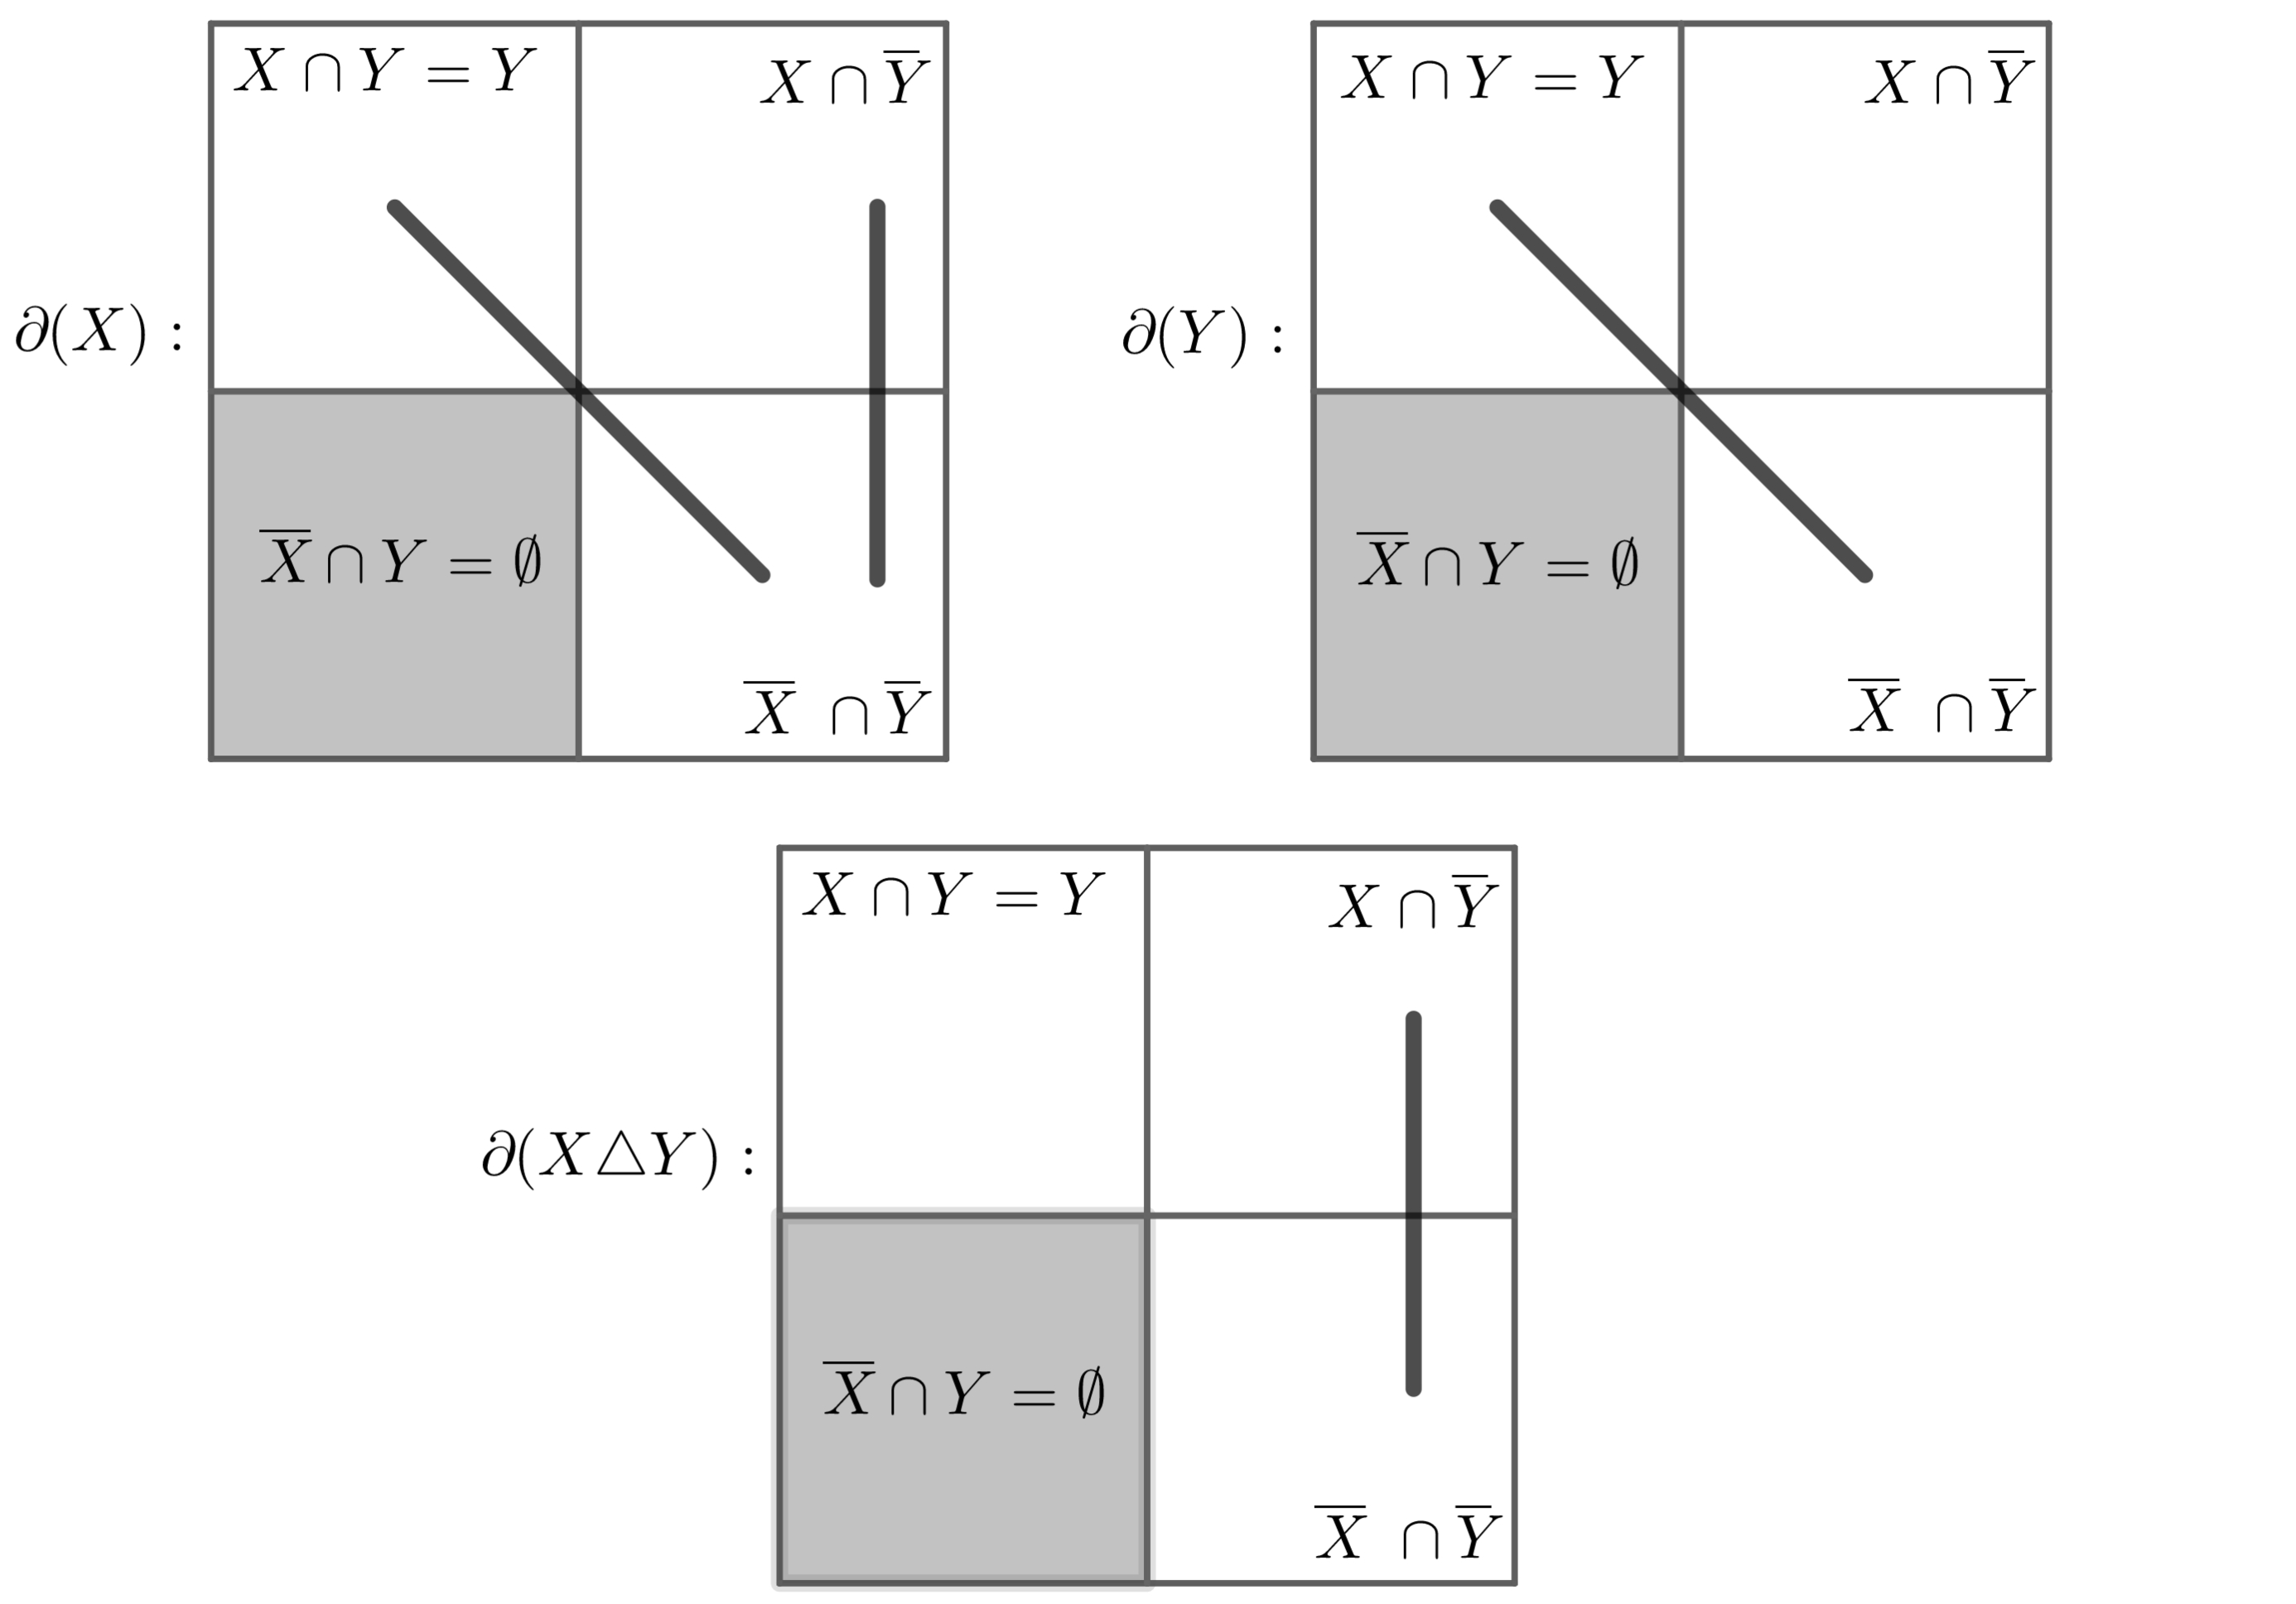
\includegraphics[width=0.8\textwidth]{img/imgchapter2/bond2.jpg}
    \caption{}
    \label{fig:bond2}
\end{figure}
Además, por el teorema \ref{teo:diferenciasimetricacortes}, $\partial(X \triangle Y)= \partial(X) \triangle \partial(Y)$. Entonces, como se muestra en la figura \ref{fig:bond2}, $\partial(X \triangle Y) = E[X \cap \overline{Y}, \overline{X} \cap \overline{Y}]$. Una vez más, la conexidad de $G$ asegura que $\partial(X \triangle Y) \neq \emptyset$. Así, en efecto, $E[X \cap \overline{Y}, \overline{X} \cap \overline{Y}] \neq \emptyset$. Esta última afirmación implica que $\partial(Y) \subsetneqq \partial(X)$. Por consiguiente, $\partial(X)$ no es un conjunto de corte minimal pues contiene propiamente a otro conjunto de corte no vacío.

Si, en segundo lugar, suponemos que $G[\bar{X}]$ no es conexa, mediante razonamientos similares podremos concluir también que $\partial(X)$ no es un conjunto de corte minimal.

La suficiencia se prueba por contradicción. Supóngase, pues, que $G[X]$ y $G[\bar{X}]$ son conexas y que $\partial(X)$ no es un conjunto de corte minimal. Entonces existe $Y \subseteq V(G)$ tal que $\partial(Y) \subsetneqq \partial(X)$ y $\partial(Y) \neq \emptyset$. Nótese que este último hecho implica que (ver la figura \ref{fig:cortessim}) $\partial(Y)= \big(E[X \cap Y, \overline{X} \cap \overline{Y}]) \bigcup (E[X \cap \overline{Y}, \overline{X} \cap Y]\big)$; de donde $$E[X \cap Y, X \cap \overline{Y}] = \emptyset = E[\overline{X} \cap Y, \overline{X} \cap \overline{Y}].$$ Sin embargo, hasta aquí nada nos garantiza que esas cuatro intersecciones (o alguna de ellas) sean no vacías. Pero, respecto a $X$ y $Y$, hay dos casos: que la intersección de $X$ con $Y$ sea vacía o no.   

\underline{Caso 1}. Asumimos que $X \cap Y = \emptyset$. Entonces $Y \subseteq \overline{X}$ y, en consecuencia, $\overline{X} \cap Y = Y$. Como $\partial(Y) \neq \emptyset$, $Y$ es no vacío; así, $\overline{X} \cap Y \neq \emptyset$. Y no podría suceder que $\overline{X} \cap \overline{Y} = \emptyset$, pues tendríamos que $\overline{X} \subseteq Y$, es decir, $\overline{X} = Y$ y, por tanto, $\partial(Y) = \partial(\overline{X})=\partial(X)$, lo cual es una contradicción.

En resumen, sabemos que $\overline{X} \cap Y \neq \emptyset$, $\overline{X} \cap \overline{Y} \neq \emptyset$ y $E[\overline{X} \cap Y, \overline{X} \cap \overline{Y}] = \emptyset$. Esto implicaría que $G[\bar{X}]$ no es conexa, y contradice nuestras hipótesis.

\underline{Caso 2}. Suponemos que $X \cap Y \neq \emptyset$. Si se cumpliera que $X \cap \overline{Y} \neq \emptyset$, $G[X]$ no sería conexa pues $E[X \cap Y, X \cap \overline{Y}] = \emptyset$, y, de nuevo, es una contradicción. Entonces debe cumplirse que $X \cap \overline{Y} = \emptyset$, o sea, que $\overline{Y} \subseteq \overline{X}$. No obstante, la consecuencia de esta última afirmación es que tanto $\overline{X} \cap Y$ como $\overline{X} \cap \overline{Y}$ son conjuntos no vacíos. 

En efecto, si $\overline{X} \cap Y = \emptyset$ sabemos que $\overline{X} \subseteq \overline{Y}$. Dado que $\overline{Y} \subseteq \overline{X}$, entonces $Y = X$ y $\partial(Y) = \partial(X)$, lo cual es imposible. Por otro lado, si se diera que $\overline{X} \cap \overline{Y} = \emptyset$, tendríamos que $\overline{Y} \subseteq X$. Como $\overline{Y} \subseteq \overline{X}$, también $X \subseteq Y$. Por consiguiente, $\overline{Y} \subseteq Y$. Esto último es falso debido a que $Y \neq \emptyset$.

Así, $\overline{X} \cap Y \neq \emptyset$ y $\overline{X} \cap \overline{Y} \neq \emptyset$. Pero, tomando en cuenta que $E[\overline{X} \cap Y, \overline{X} \cap \overline{Y}] = \emptyset$, tendríamos que $G[\bar{X}]$ no es conexa, una contradicción.

Podemos asegurar que los casos anteriores no son posibles. Las dificultades surgieron a partir de que supusimos que $\partial(X)$ no es un conjunto de corte minimal.

Concluímos, finalmente, que $\partial(X)$ es un conjunto de corte minimal si y sólo si $G[X]$ y $G[\bar{X}]$ son conexas. 

\end{proof}

En general, un conjunto de corte \textit{divide} a $G$ en, al menos, dos componentes conexas. No obstante, el teorema anterior nos asegura, pues, que los cortes minimales son aquellos que dividen a $G$ en, e\textit{exactamente}, dos componentes.

\begin{figure}[H]
    \centering
    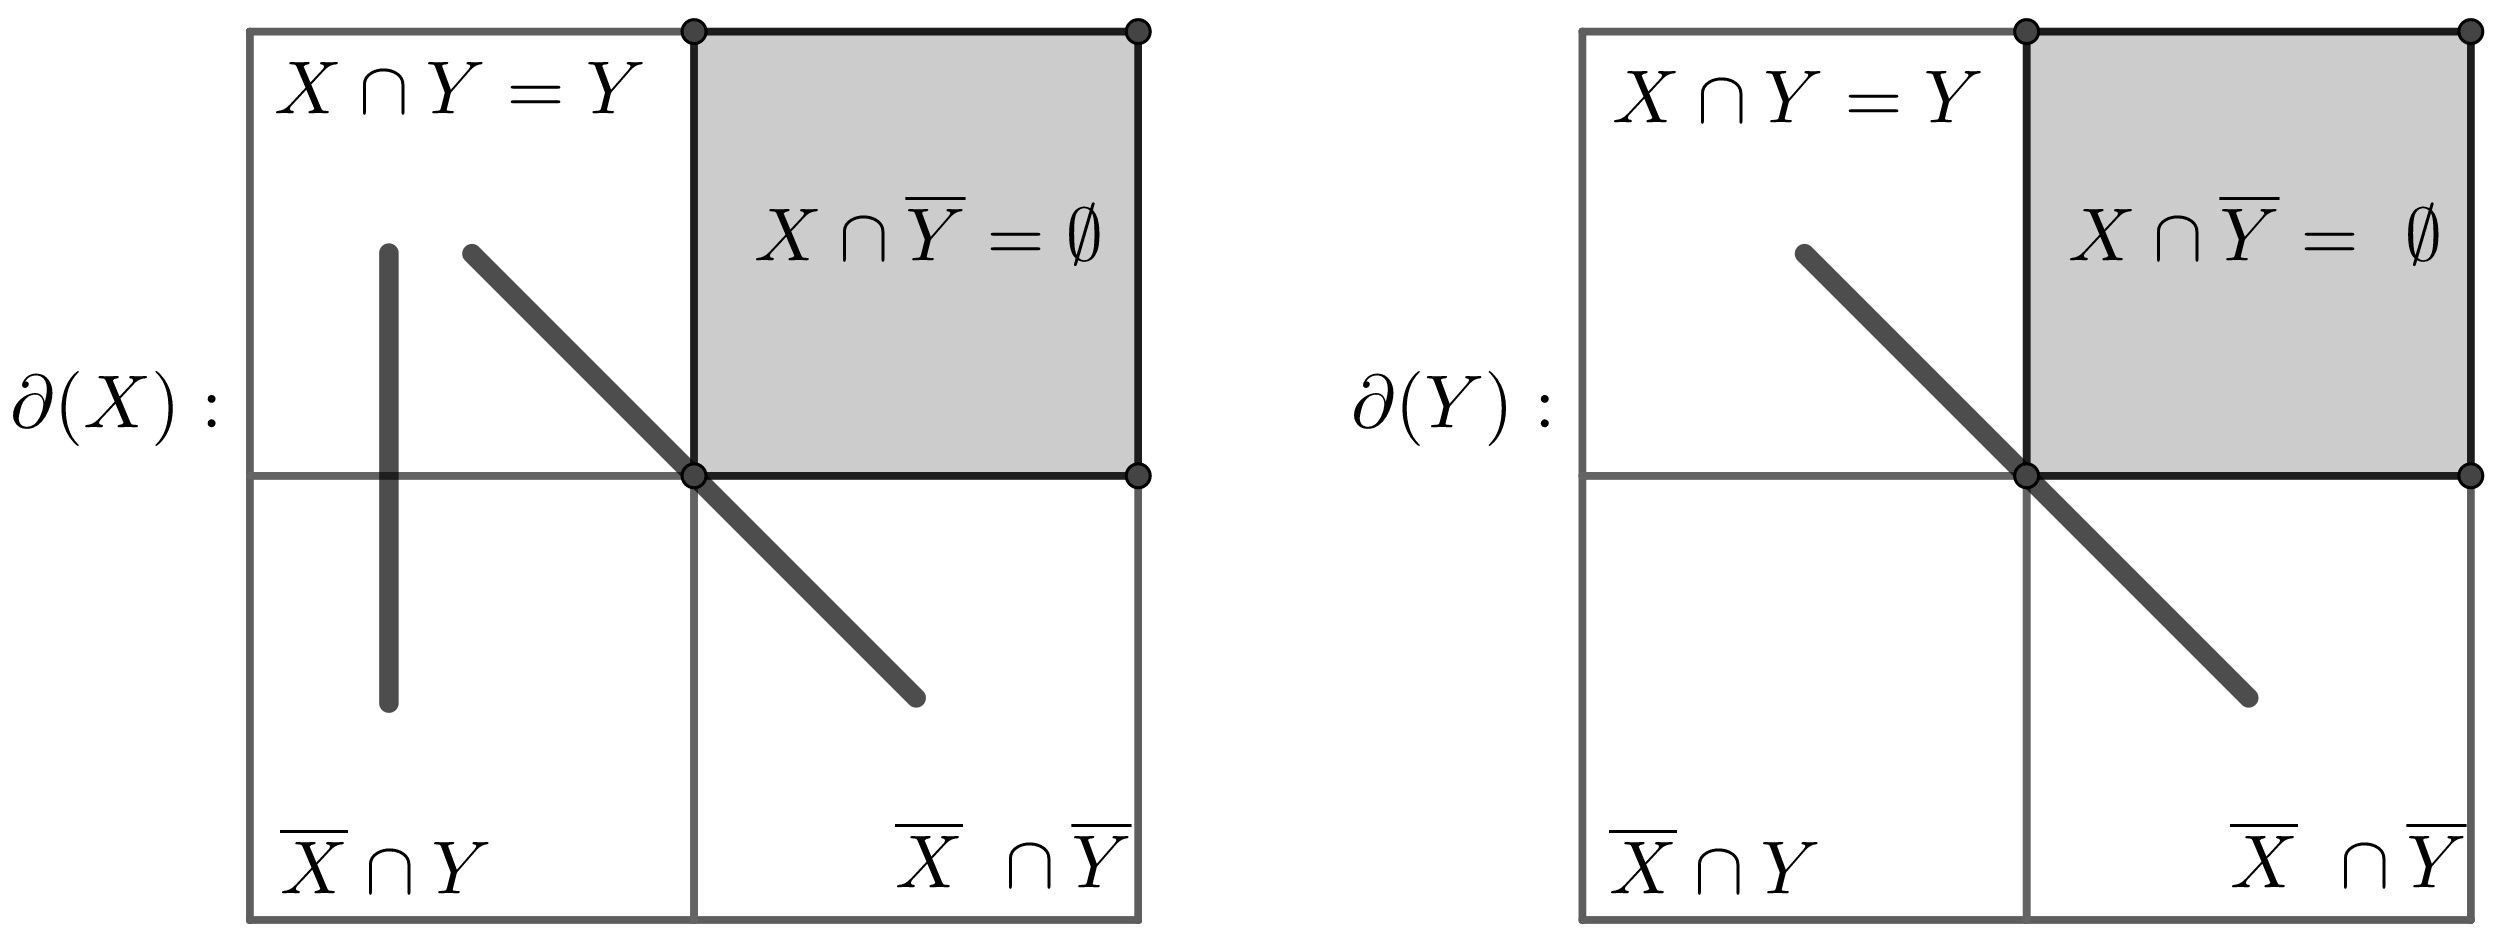
\includegraphics[scale=0.2]{img/imgchapter2/bondvertices.jpg}
    \caption{}
    \label{fig:bondvertices}
\end{figure}
Si $B$ es un corte minimal contenido en $\partial(X)$, una forma de hallar el conjunto de vértices $Y$ tal que $B = \partial(Y)$ es así: como $B$ es minimal, $G\setminus B$ consta de dos componentes conexas, digamos $F_{1}$ y $F_{2}$. Por otro lado, dada cualquier arista $e \in B$, forzosamente tiene un extremo en $X$ y otro en $\overline{X}$. El conjunto de éstos últimos debe estar contenido en el conjunto de vértices de alguna componente conexa, digamos, $V(F_{2})$. Entonces sucede que $V(F_{2})\cap X = \emptyset$ (si no, $G\setminus B$ es conexa). Luego, $V(F_{2})\subseteq \overline{X}$ Y $X \subseteq V(F_{1})$. Haciendo $Y:=V(F_{1})$ (y, por lo tanto, $\overline{Y}:=V(F_{2})$), es fácil comprobar que $B = \partial(Y)$.

Dado que $X \cap \overline{Y} = \emptyset$, una consecuencia de la construcción anterior es que,  $B = \partial(Y) = E[X\cap Y, \overline{X} \cap \overline{Y}]$. Además, $\partial(X) = E[X\cap Y, \overline{X} \cap \overline{Y}] \cup E[X \cap Y, \overline{X} \cap Y]$. En la imagen \ref{fig:bondvertices} representamos estas ideas al estilo de la figura \ref{fig:cortessim}.

\begin{ejem}
En la figura que se muestra a continuación están todos los conjuntos de corte minimales de la gráfica $W_{4}$. Observe que si retiráramos de $W_{4}$ las aristas de cualquiera de estos conjuntos de corte, nos quedarían dos componentes conexas, como lo asegura el teorema anterior.

\begin{figure}[H]
    \centering
    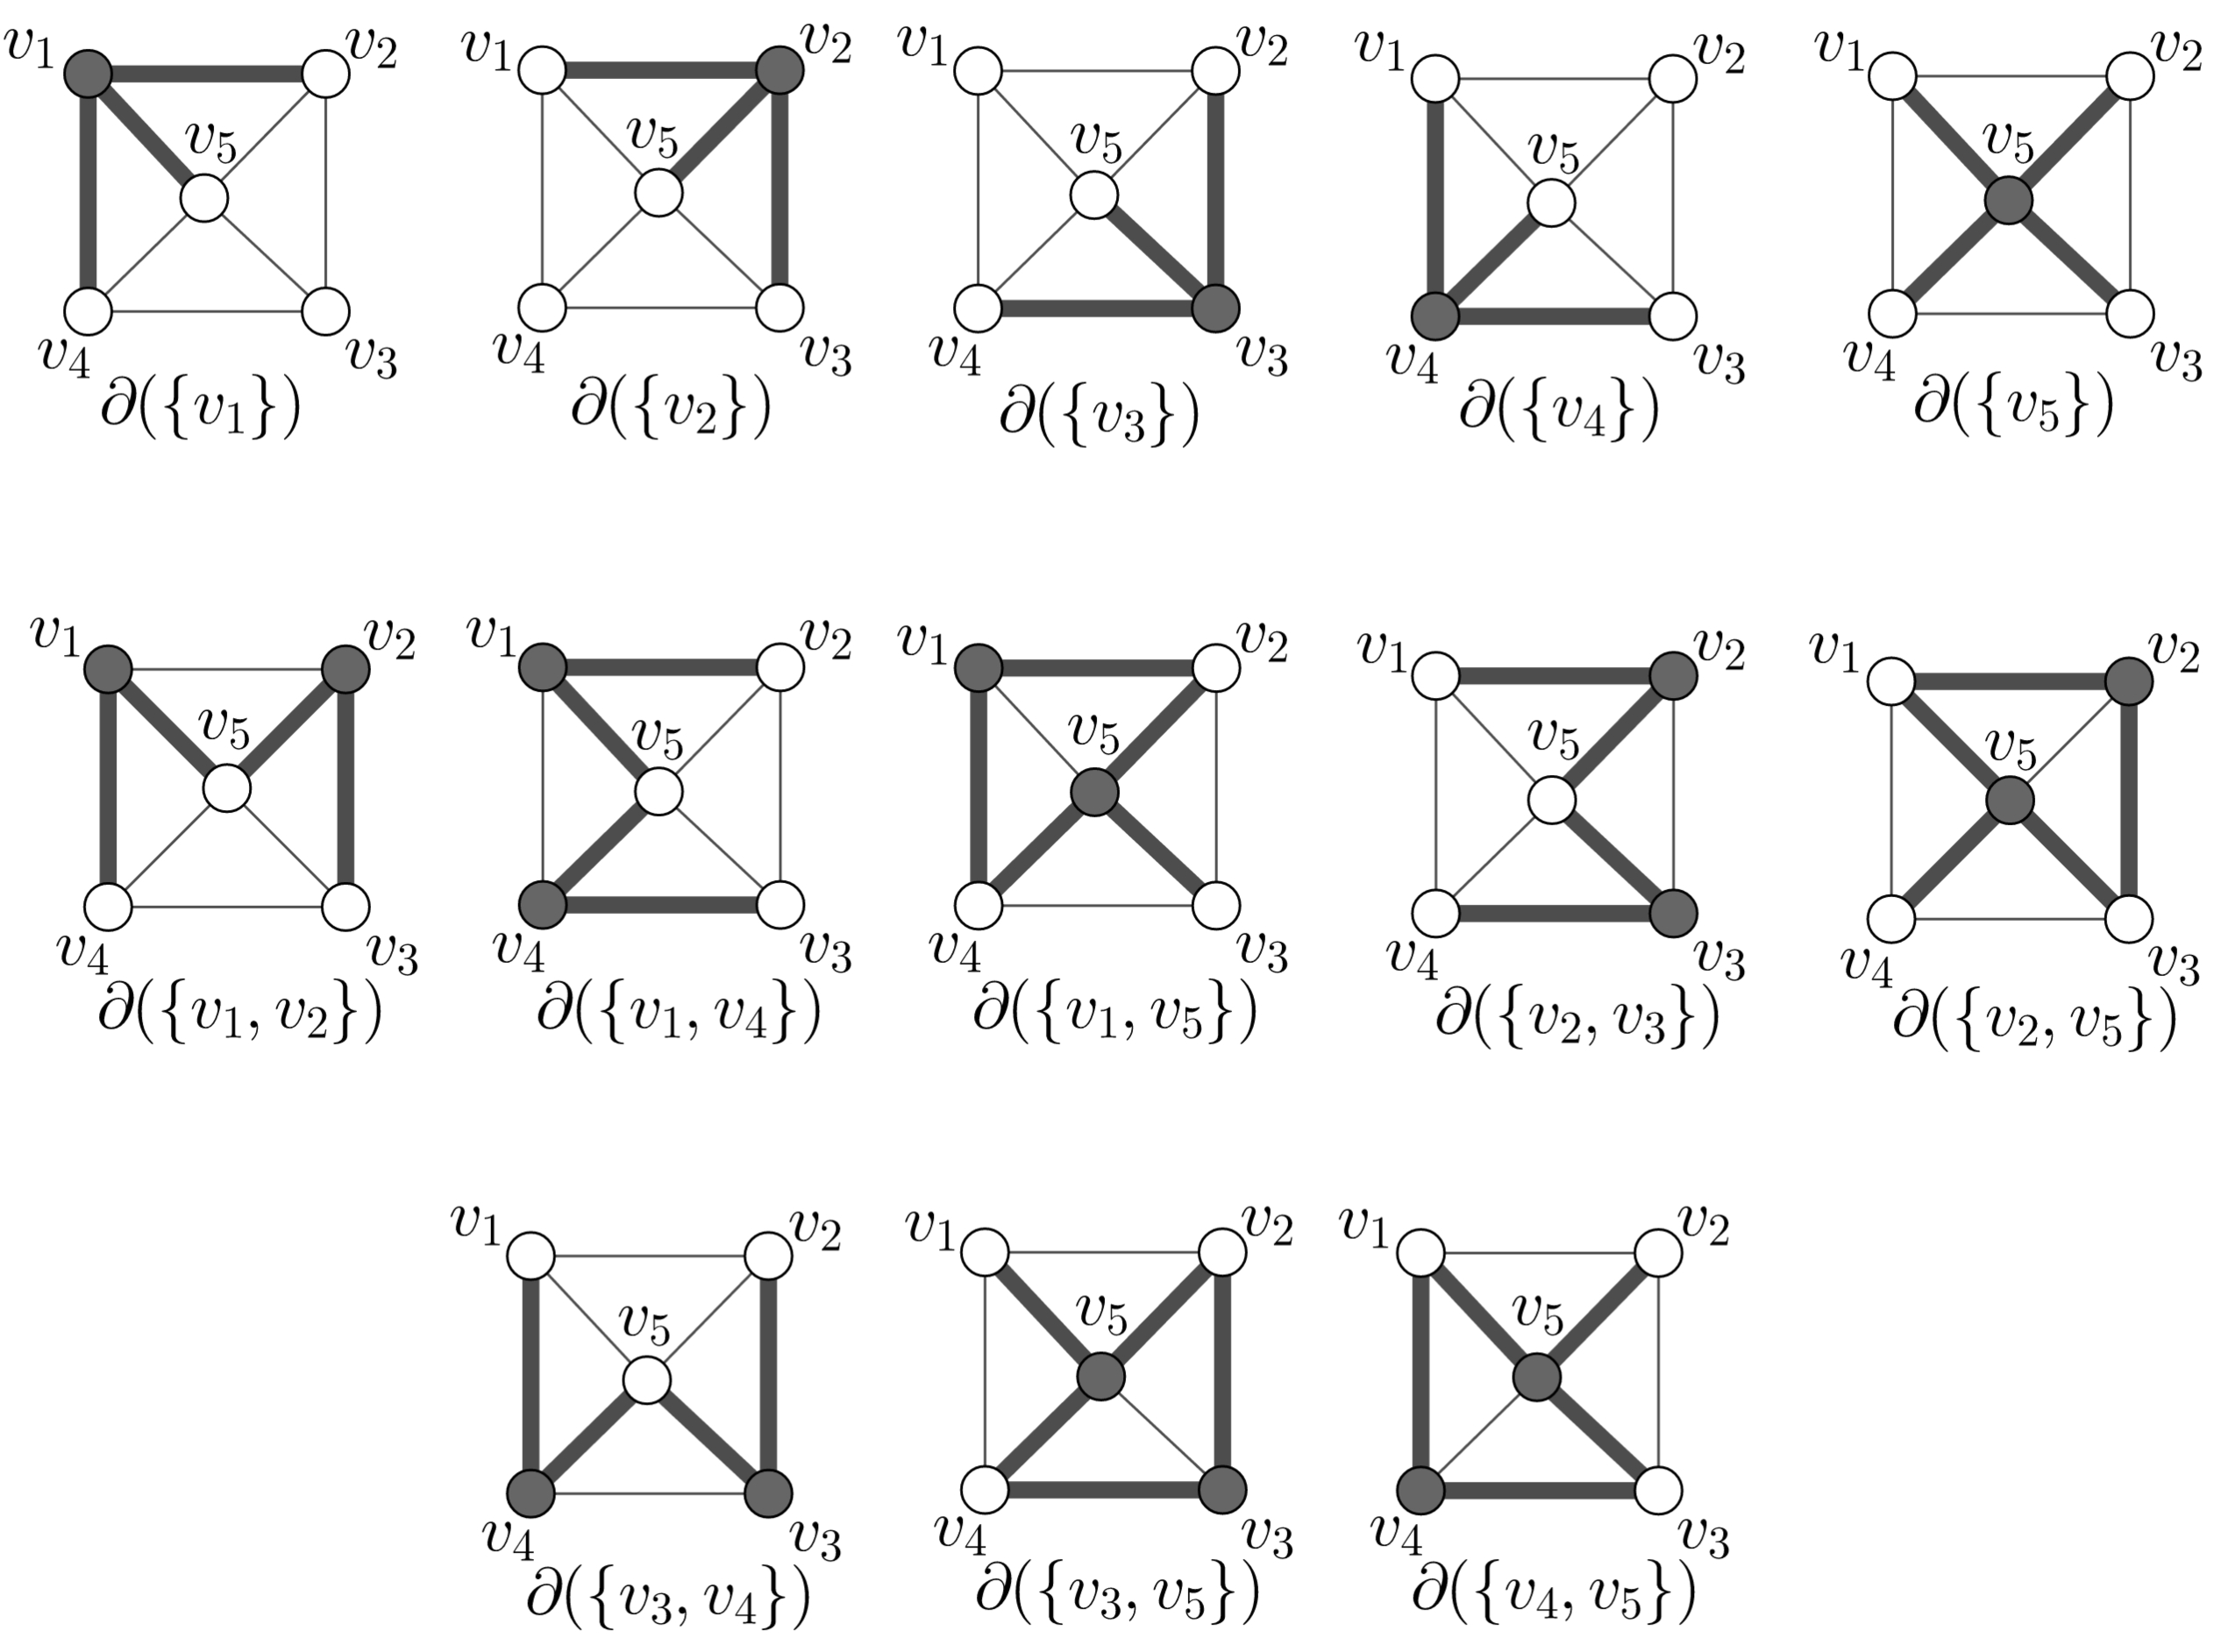
\includegraphics[width=1\textwidth]{img/imgchapter2/bond.jpg}
    \caption{Conjuntos de corte minimales de $W_{4}$}
    \label{fig:bondw4}
\end{figure}

\hfill $\blacklozenge$
\end{ejem}

En suma, el teorema \ref{teo:caracterizacionbond} indica que \textit{$\partial(X)$ es un conjunto de corte minimal si y sólo si $G\setminus \partial(X)$ tiene exactamente dos componentes conexas}. ¿Qué relación tienen los conjuntos de corte minimales y aquellos que no lo son? El siguiente teorema responde esta cuestión. 

\begin{teo}\label{teo:unionajenademinimales}
Sea $G$ una gráfica. Una subgráfica generadora de $G$ es un conjunto de corte si y sólo si es es unión ajena de conjuntos de corte minimales.
\end{teo}

\begin{proof}
Supongamos que $S \subseteq G$ es un conjunto de corte. Si $S$ ya es minimal, terminamos. Si no, $S$ contiene a un conjunto de corte minimal, digamos $B_{1}$. Entonces, claramente, $S=B_{1} \cup (S \setminus B_{1})$. De nuevo, si $S \setminus B_{1}$ es un conjunto de corte minimal, terminamos. Si no es así, tomamos un minimal $B_{2} \subseteq (S \setminus B_{1})$ y observamos que $S=B_{1} \cup B_{2} \cup (S \setminus (B_{1} \cup B_{2}))$. Nos preguntamos si $S \setminus (B_{1} \cup B_{2})$ es minimal o no y repetimos el mismo procedimiento anterior hasta terminar en un $q$-ésimo paso de tal forma que $B_{q} = S \setminus (B_{1} \cup \ldots \cup B_{q-1})$ sea un conjunto de corte minimal. Así, $S=B_{1} \cup \ldots \cup B_{q}$, y esta unión es ajena por construcción.

Asumimos ahora que $S=B_{1} \cup \ldots \cup B_{q}$ es unión ajena de conjuntos de corte minimales. Como cada $B_{i}$ es un corte, ya argumentamos que existe $Y_{i} \subseteq V(G)$ tal que $B_{i} = \partial(Y_{i})$. Luego, $S = \partial(Y_{1}) \cup \ldots \cup \partial(Y_{q})$. Sin embargo, la unión es ajena por hipótesis y, así, se tiene que $S=\partial(Y_{1}) \triangle \ldots \triangle \partial(Y_{q})$. Utilizando el teorema \ref{teo:diferenciasimetricacortes}, deducimos que $S=\partial(Y_{1} \triangle \ldots \triangle Y_{q})$. Por lo tanto, $S$ es un conjunto de corte.

Concluímos que $S \subseteq G$ es un conjunto de corte si y sólo si es es unión ajena de conjuntos de corte minimales.  

\end{proof}


\subsection{Conjuntos de corte fundamentales}
Sea $T$ un árbol generador de $G$. Es común referirse a las aristas de $T$ como \textit{ramas}. Asimismo, llamamos \textit{coárbol} al complemento de $T$ respecto a $G$, es decir, a la subgráfica generadora de $G$ cuyas aristas están determinadas por el conjunto $E(G)\setminus E(T)$. Lo denotamos como $\overline{T}$ y a sus aristas las llamamos \textit{cuerdas de} $T$.

\begin{prop}\label{prop:bondintersection}
Dado cualquier árbol generador $T$ de $G$y cualquier conjunto de corte $\partial(X) \neq \varnothing$ de $G$, siempre sucede que $\partial(X) \cap T \neq \varnothing$.

\end{prop}

\begin{proof}
Supongamos que $\partial(X) \cap T = \varnothing$. Entonces $B \subseteq \overline{T}$, de donde $T = G\setminus T \subseteq G \setminus B$. Sin embargo, $G\setminus B$ es inconexa y $T$ es un árbol generador que es conexo (porque $G$ es conexa), lo cual es una contradicción. Por lo tanto, $B \cap T \neq \varnothing$ 

\end{proof}

La proposición anterior implica que  $\varnothing$ es el único conjunto de corte tal que  $\varnothing \subseteq \overline{T}$, es decir, que el corte vacío es el único conjunto de corte que está contenido en el coárbol $\overline{T}$.

Sea $b$ una rama cualquiera de $T$. Dado que $T \setminus \{b\}$ es inconexa, debe existir $X \subseteq V(T)=V(G)$ tal que $\partial_{T}(X) = \{b\}$. Observemos, por cómo está construido, que el corte $\partial_{G}(X)$ está contenido en $\overline{T}+b$. Esto asegura que $G \setminus \partial(X)$ está constituido por dos componentes conexas. Así, $\partial_{G}(X)$ es un corte minimal. Además, tal corte es único con la propiedad de estar contenido en $\overline{T}+b$. En efecto, digamos que hay otro $B \subseteq \overline{T} + b$. Luego,
\begin{align*}
(\partial_{G}(X) \triangle B) \cap T &= (\partial_{G}(X) \cap T)\triangle(B\triangle T)\\
&= b \triangle b \\
&= \varnothing.
\end{align*}
Pero lo anterior se da sólo si $\partial_{G}(X)\triangle B \subseteq \overline{T}$. Como el único conjunto de corte contenido en el coárbol es la gráfica vacía, entonces $\partial_{G}(X)\triangle B = \varnothing$, i.e., $\partial_{G}(X)=B$. Por tanto, $\partial_{G}(X)$ es el único corte con la propiedad de estar contenido en $\overline{T}+b$.

Así que $\partial_{G}(X)$ es llamado el\textit{conjunto de corte fundamental de} $G$ con respecto a $T$ y a $b$ y será frecuente denotarlo como $\mathscr{B}_{b}$ (quedando el árbol generador implícito). Es claro que árboles generadores distintos darán lugar a cortes fundamentales distintos. 

\begin{prop}\label{cortesfundamentalespropchida}
Sea $S \subseteq T$ una subgráfica generadora de $G$. Consideremos  
$$
B =\difsym_{b \in E(S)} \mathscr{B}_{b}. 
$$
Entonces $B$ es un conjunto de corte. Además, $B \cap T = S$ y $B$ es el único conjunto de corte de $G$ con esta propiedad.
\end{prop}

\begin{proof}
Que $B$ sea un conjunto de corte se da por el teorema \ref{teo:diferenciasimetricacortes}. Por otro lado, nótese que
\begin{align*}
    B \cap T &=(\difsym_{b \in E(S)} \mathscr{B}_{b}) \cap T \\
             &=\difsym_{b \in E(S)} (\mathscr{B}_{b} \cap T) \\
             &=\difsym_{b\in E(S)} b \\
             &= S.
\end{align*}
Además, si hubiese otro corte $B'$ tal que $B' \cap T= S$, entonces $(B \triangle B') \cap T = \varnothing$. Así, $B \triangle B' \subseteq \overline{T}$ y $B = B'$, y $B$ es único.

\end{proof}

\begin{cor} \label{basecortesfundamentales}
Todo conjunto de corte de $G$ puede expresarse de manera única como una diferencia simétrica de conjuntos de corte fundamentales con respecto a $T$.
\end{cor}

\begin{proof}
Sea $\partial(X)$ un conjunto de corte cualquiera de $G$. Hacemos $S= \partial(X) \cap T$. Por el teorema anterior, necesariamente, $\partial(X) = \difsym_{b \in E(S)} \mathscr{B}_{B}$ y es el único con tales propiedades.

\end{proof}

Por el capítulo previo, sabemos que $T$ tiene $n-1$ ramas, lo que significa que, necesariamente, $G$ debe contener $n-1$ cortes fundamentales respecto a $T$.

\begin{ejem} \label{ejem:cortesfundamentales}
Recuérdese la gráfica rueda $W_{4}$ de la figura \ref{fig:wheel}. En la imagen \ref{fig:bondminimales}, en el inciso $(a)$, tomamos un árbol generador $T$ cuyas aristas son $\{a, d, e, g\}$. En el inciso $(b)$ mostramos dos cortes fundamentales, uno respecto a la rama $g$ y el otro respecto a $e$.

\begin{figure}[t]
    \centering
    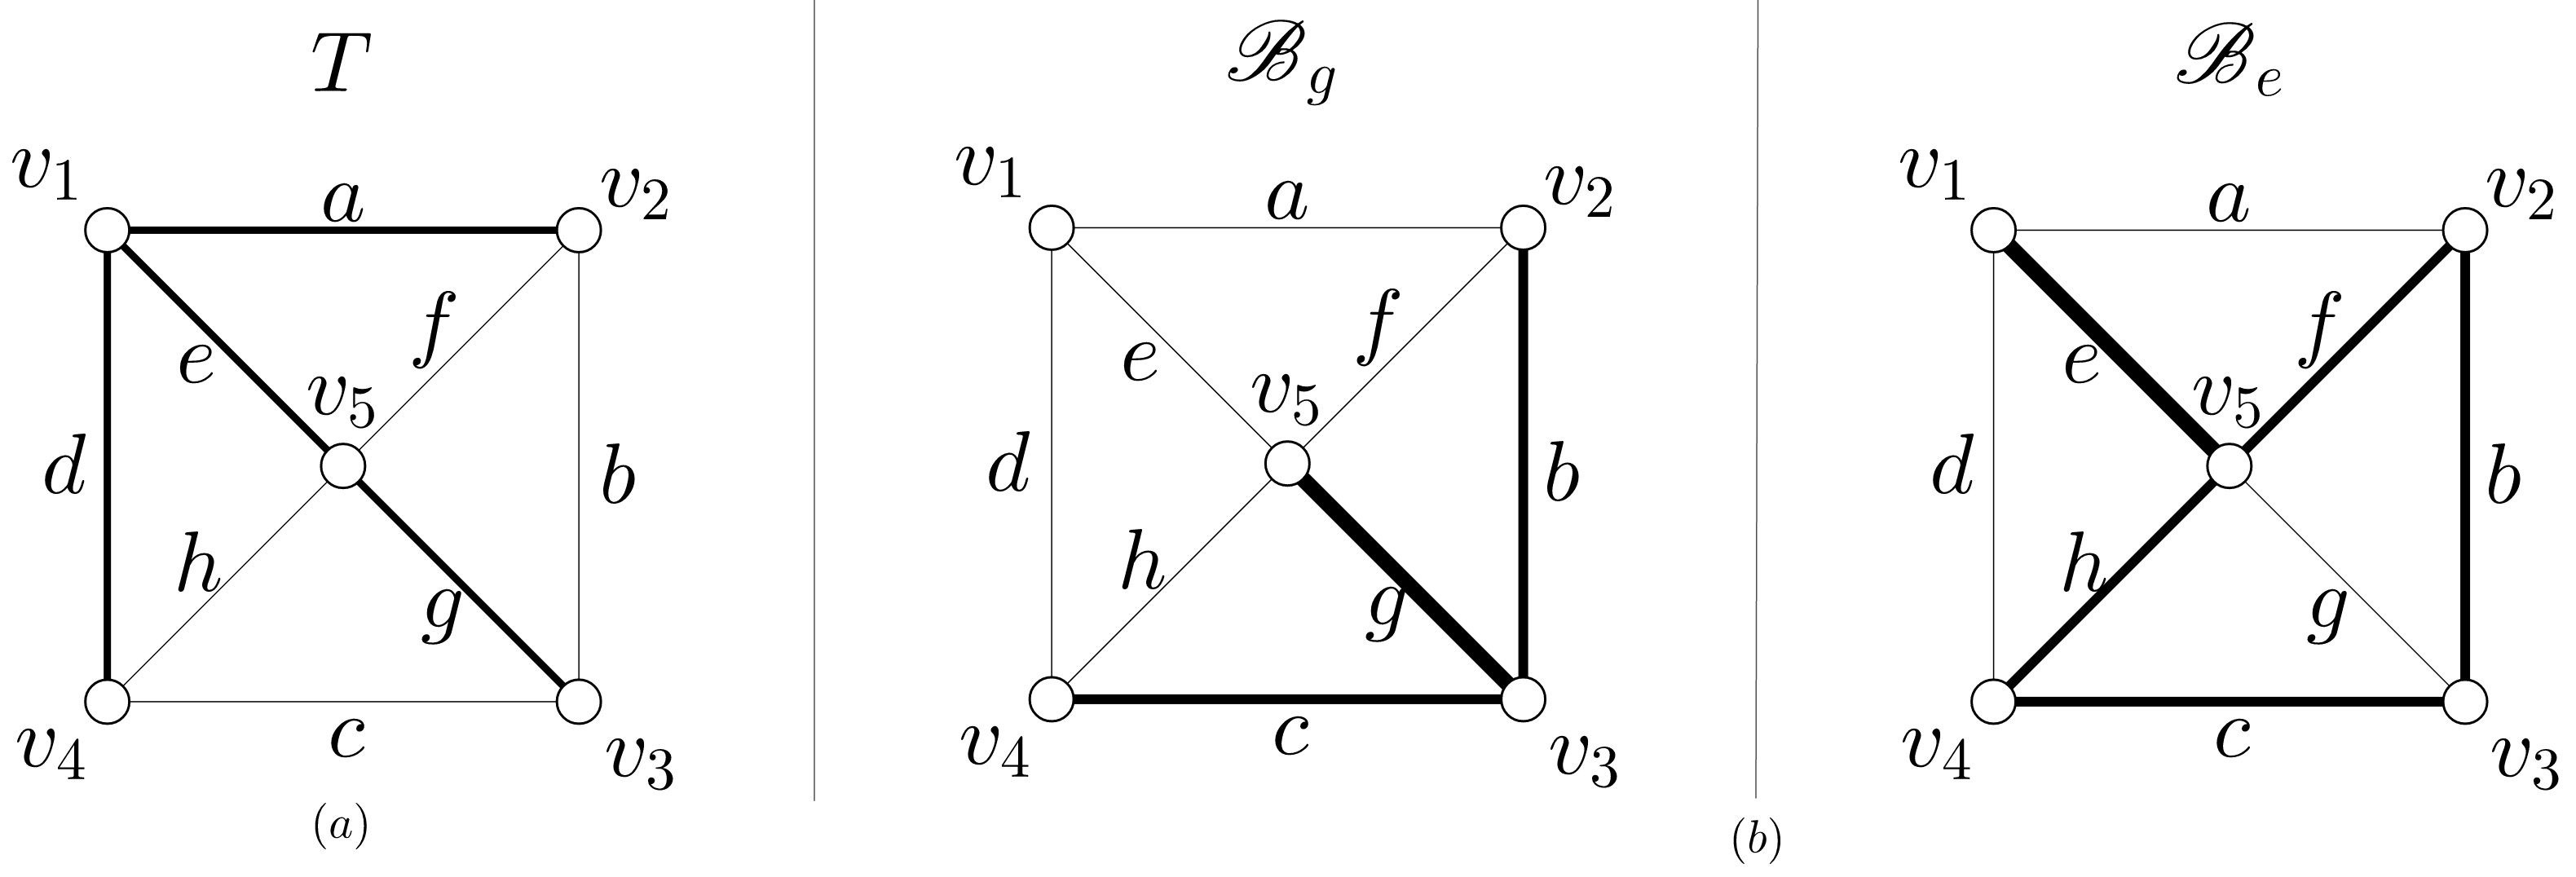
\includegraphics[scale = 0.15]{img/imgchapter2/bondminimales.jpg}
    \caption{}
    \label{fig:bondminimales}
\end{figure}

\hfill $\blacklozenge$
\end{ejem}



\section{Gráficas pares de $G$}
Decimos que una gráfica es \textit{par} si y sólo si todos sus vértices tienen grado par. En particular, los ciclos son gráficas pares pues todos sus vértices tiene grado $2$; así como la gráfica vacía $\varnothing$, cuyos vértices tienen grado $0$. Ahora nos enfocaremos en estudiar las subgráficas generadoras pares de $G$. Primero probaremos algunos resultados que relacionan a los conjuntos de corte con las gráficas pares.  Comenzamos con el siguiente lema.

\begin{lema} \label{lema1}
Si $X \subseteq V(G)$, entonces
$$
\big|\partial(X)\big|= \sum _{v \in X} d(v)- 2 \big |E[X]\big |.
$$
\end{lema}

\begin{proof} Para esta prueba haremos uso de su matriz de incidencia $\mathbf{M}_{G}$.

Basándonos en las ideas que expusimos en el capítulo anterior, sabemos que se cumple:
\begin{equation} \label{eq4}
\sum_{v \in X} \sum_{e \in E(G)} m_{ve} = \sum_{e \in E(G)} \sum_{v \in X} m_{ve}.
\end{equation}

Se sabe también que $\sum_{e \in E(G)} m_{ve} = d(v)$, con $v \in X$. Así, en particular, 
\begin{equation} \label{eq5}
    \sum_{v \in X} \sum_{e \in E(G)} m_{ve} =\sum_{v \in X} d(v).
\end{equation}

Por otro lado, es sencillo darse cuenta que el conjunto de aristas se particiona de la siguiente manera: $E(G)=\partial(X) \cup E[X] \cup E[\bar{X}]$. De aquí, dada una arista $e \in E(G)$, y de la definción de $\mathbf{M}_{G}$, se tiene
 $$
  \sum_{v \in X} m_{ve} = \left\{\begin{matrix}
1, & \text{si} \hspace{1.5mm} e \in \partial(X) \\ 
2, & \text{si} \hspace{1.5mm} e \in E[X]        \\
0, & \text{si} \hspace{1.5mm} e \in E[\bar{X}]
\end{matrix}\right..
 $$
 Luego, deducimos que:
  $$
  \sum_{e \in E(G)} \sum_{v \in X} m_{ve} = \sum_{e \in \partial(X)} \big( \sum_{v \in X} m_{ve} \big) + \sum_{e \in E[X]} \big(\sum_{v \in X} m_{ve}\big) + \sum_{e \in E[\bar{X}]} \big(\sum_{v \in X} m_{ve}\big).
  $$
  Por tanto, 
  \begin{equation} \label{eq6}
      \sum_{e \in E(G)} \sum_{v \in X} m_{ve} = \big| \partial(X) \big| + 2 \big| E[X] \big|.
  \end{equation}
  Sustituyendo las ecuaciones \ref{eq5} y \ref{eq6} en \ref{eq4}, y realizando las operaciones adecuacada, llegamos a la igualdad deseada: $\big|\partial(X)\big|= \sum _{v \in X} d(v)- 2 \big |E[X]\big |$.
  
  
\end{proof}

\begin{prop} \label{prop2}
Sean $H_{1}, H_{2}$ subgráficas pares de $G$. Si $X \subseteq V(G)$, entonces 
$$
\partial_{H_{1} \triangle H_{2}}(X) = \partial_{H_{1}}(X) \triangle \partial_{H_{2}}(X).
$$
\end{prop}

\begin{proof} Lo haremos por \textit{doble contención}. Para la primer contención, tomamos $a \in \partial_{H_{1} \triangle H_{2}}(X)$. Entonces la arista $a$ es adyacente a dos vértices: $u$ y $v$; asumiremos (sin pérdida de generalidad) que el primero está en $X$ y el otro en $\overline{X}$. Entonces $a \in E(H_{1} \triangle H_{2})=E(H_{1}) \triangle E(H_{2})$. Si $a$ está en $E(H_{1})$ (y no a $E(H_{2})$), necesariamente $a$ pertenece a $\partial_{H_{1}}(X)$ por cómo son los vértices de $a$. No sucede que $a \in \partial_{H_{2}}(X)$ porque $a \notin E(H_{2})$. Similarmente, si $a$ es elemento de $E(H_{2})$ (y no de $E(H_{1})$), entonces $a \in \partial_{H_{2}}(X)$ y no pertenece a $\partial_{H_{1}}(X)$. Por tanto, $a \in \partial_{H_{1}}(X) \triangle \partial_{H_{2}}(X)$. De esta manera, hallamos que $\partial_{H_{1} \triangle H_{2}}(X) \subseteq \partial_{H_{1}}(X) \triangle \partial_{H_{2}}(X)$.

Ahora suponemos que la arista $a$ pertenece al conjunto $\partial_{H_{1}}(X) \triangle \partial_{H_{2}}(X)$. Por la definición de la \textit{diferencia simétrica} existen dos casos.

\underline{Caso 1}: Supongamos que $a$ pertenece a $\partial_{H_{1}}(X)$ (y, por tanto, no es elemento de $\partial_{H_{2}}(X)$). Entonces $a \in E(H_{1})$. No es posible que $a \in E(H_{2})$, pues, inmeditamente, $a$ estaría en $\partial_{H_{2}}(X)$ ya que $u \in X$ y $v \in \overline{X}$, y aquello es una contradicción. Por consiguiente, $a \in E(H_{1}) \triangle E(H_{2}) = E(H_{1} \triangle H_{2})$. Dado que un extremo de la arista está en $X$ y el el otro en el complemento de $X$, deducimos que $a \in \partial_{H_{1} \triangle H_{2}}(X)$.

\underline{Caso 2}: Supongamos que $a$ pertenece a $\partial_{H_{2}}(X)$ (y, por tanto, no es elemento de $\partial_{H_{1}}(X)$). Procediendo de forma análoga al caso anterior obtenemos, también, que $a \in \partial_{H_{1} \triangle H_{2}}(X)$.

De ambos casos, afirmamos que $\partial_{H_{1}}(X) \triangle \partial_{H_{2}}(X) \subseteq \partial_{H_{1} \triangle H_{2}}(X)$.

Concluímos, pues, que $\partial_{H_{1} \triangle H_{2}}(X) = \partial_{H_{1}}(X) \triangle \partial_{H_{2}}(X)$.

\end{proof}


\begin{prop} \label{prop3}
$G$ es par si y sólo si $|\partial(X)|$ es par, para cualquier $X \subseteq V(G)$.
 
\end{prop}

\begin{proof}
Supongamos que $G$ es par y sea $X$ un subconjunto de vértices de $G$. De la paridad de $G$ se deduce que $\sum_{v \in X} d(v)$ es par. Luego entonces $\sum _{v \in X} d(v)- 2 \big |E[X]\big |$ es par y, por el lema \ref{lema1}, $\big|\partial(X)\big|$ también es par.

En segundo lugar, asumimos que $\big|\partial(X)\big|$ es par, con $X$ cualquier subconjunto de vértices de $G$. En particular, dado $v \in V(G)$, $\big|\partial(\{v\})\big|$ es par. En la sección pasada mencionamos que en $\partial(\{v\})$ se encuentran todas las aristas que inciden en $v$, excepto sus posibles lazos. Si $\partial(\{v\}) = \emptyset$ y $v$ no tiene lazos, entonces su grado es cero. Si $v$ tiene lazos, recordemos que estos se cuentan doble para el grado, de forma que éste sería par de todos modos. Si, ahora, $\partial(\{v\}) \neq \emptyset$, como $\big| \partial(\{v\}) \big|$ es par, inciden en $v$ un cantidad par de aristas y, si tuviera lazos, éstos se cuentan doble, de tal manera que $d(v)$ es un número par. Por lo tanto, todos los vértices de $G$ tienen grado par, i.e., $G$ es par.

Luego, $G$ es par si y sólo si, para todo $X \subseteq V(G)$, $|\partial(X)|$ es par.

\end{proof}

Para la demostración del siguiente teorema es necesario recordar que $|A \triangle B| = |A|+|B| - 2|A \cap B|$.

\begin{teo} \label{teo:difsimciclos}
 Dada $G$ una gráfica, la diferencia simétrica de dos subgráficas pares de $G$ es también una subgráfica par de $G$.
\end{teo}

\begin{proof}
Sean $C_{1}, C_{2}$ dos subgráficas pares cualesquiera de $G$. Tomamos un subconjunto $X$ de vértices de $G$. Por la proposición \ref{prop2}, es cierto que 
$$\partial_{C_{1} \triangle C_{2}}(X) = \partial_{C_{1}}(X) \triangle \partial_{C_{2}}(X).$$
Además, en virtud de la proposición \ref{prop3}, $|\partial_{C_{1}}(X)|$ y $|\partial_{C_{2}}(X)|$ son números pares. Entonces 
$$|\partial_{C_{1}}(X) \triangle \partial_{C_{2}}(X)| = |\partial_{C_{1}}(X)| + |\partial_{C_{2}}(X)| - 2 |\partial_{C_{1}}(X) \cap \partial_{C_{2}}(X)|$$
es también un número par, es decir, $\partial_{C_{1} \triangle C_{2}}(X)$ tiene cardinalidad par. De nuevo por la proposición \ref{prop3}, concluímos que $C_{1} \triangle C_{2}$ es una subgráfica par.

\end{proof}

\subsection{Los ciclos de $G$}
De acuerdo a nuestro contexto, puesto que estamos tratando con las subgráficas generadoras de $G$, un \textit{ciclo de} $G$ es una subgráfica generadora de $G$ cuyas aristas forman un sólo ciclo (en el sentido de la definición dada en el capítulo $1$). Dicho de otra manera, en lo que sigue, un \textit{ciclo de} $G$ es una subgráfica par de $G$ cuyos vértices son de grado $2$ ó $0$.

\begin{ejem}
En la figura \ref{fig:espaciociclos} se encuentran todas las subgráficas pares de la gráfica $W_{4}$ y hemos resaltado sus respectivas aristas.

\begin{figure}[H]
    \centering
    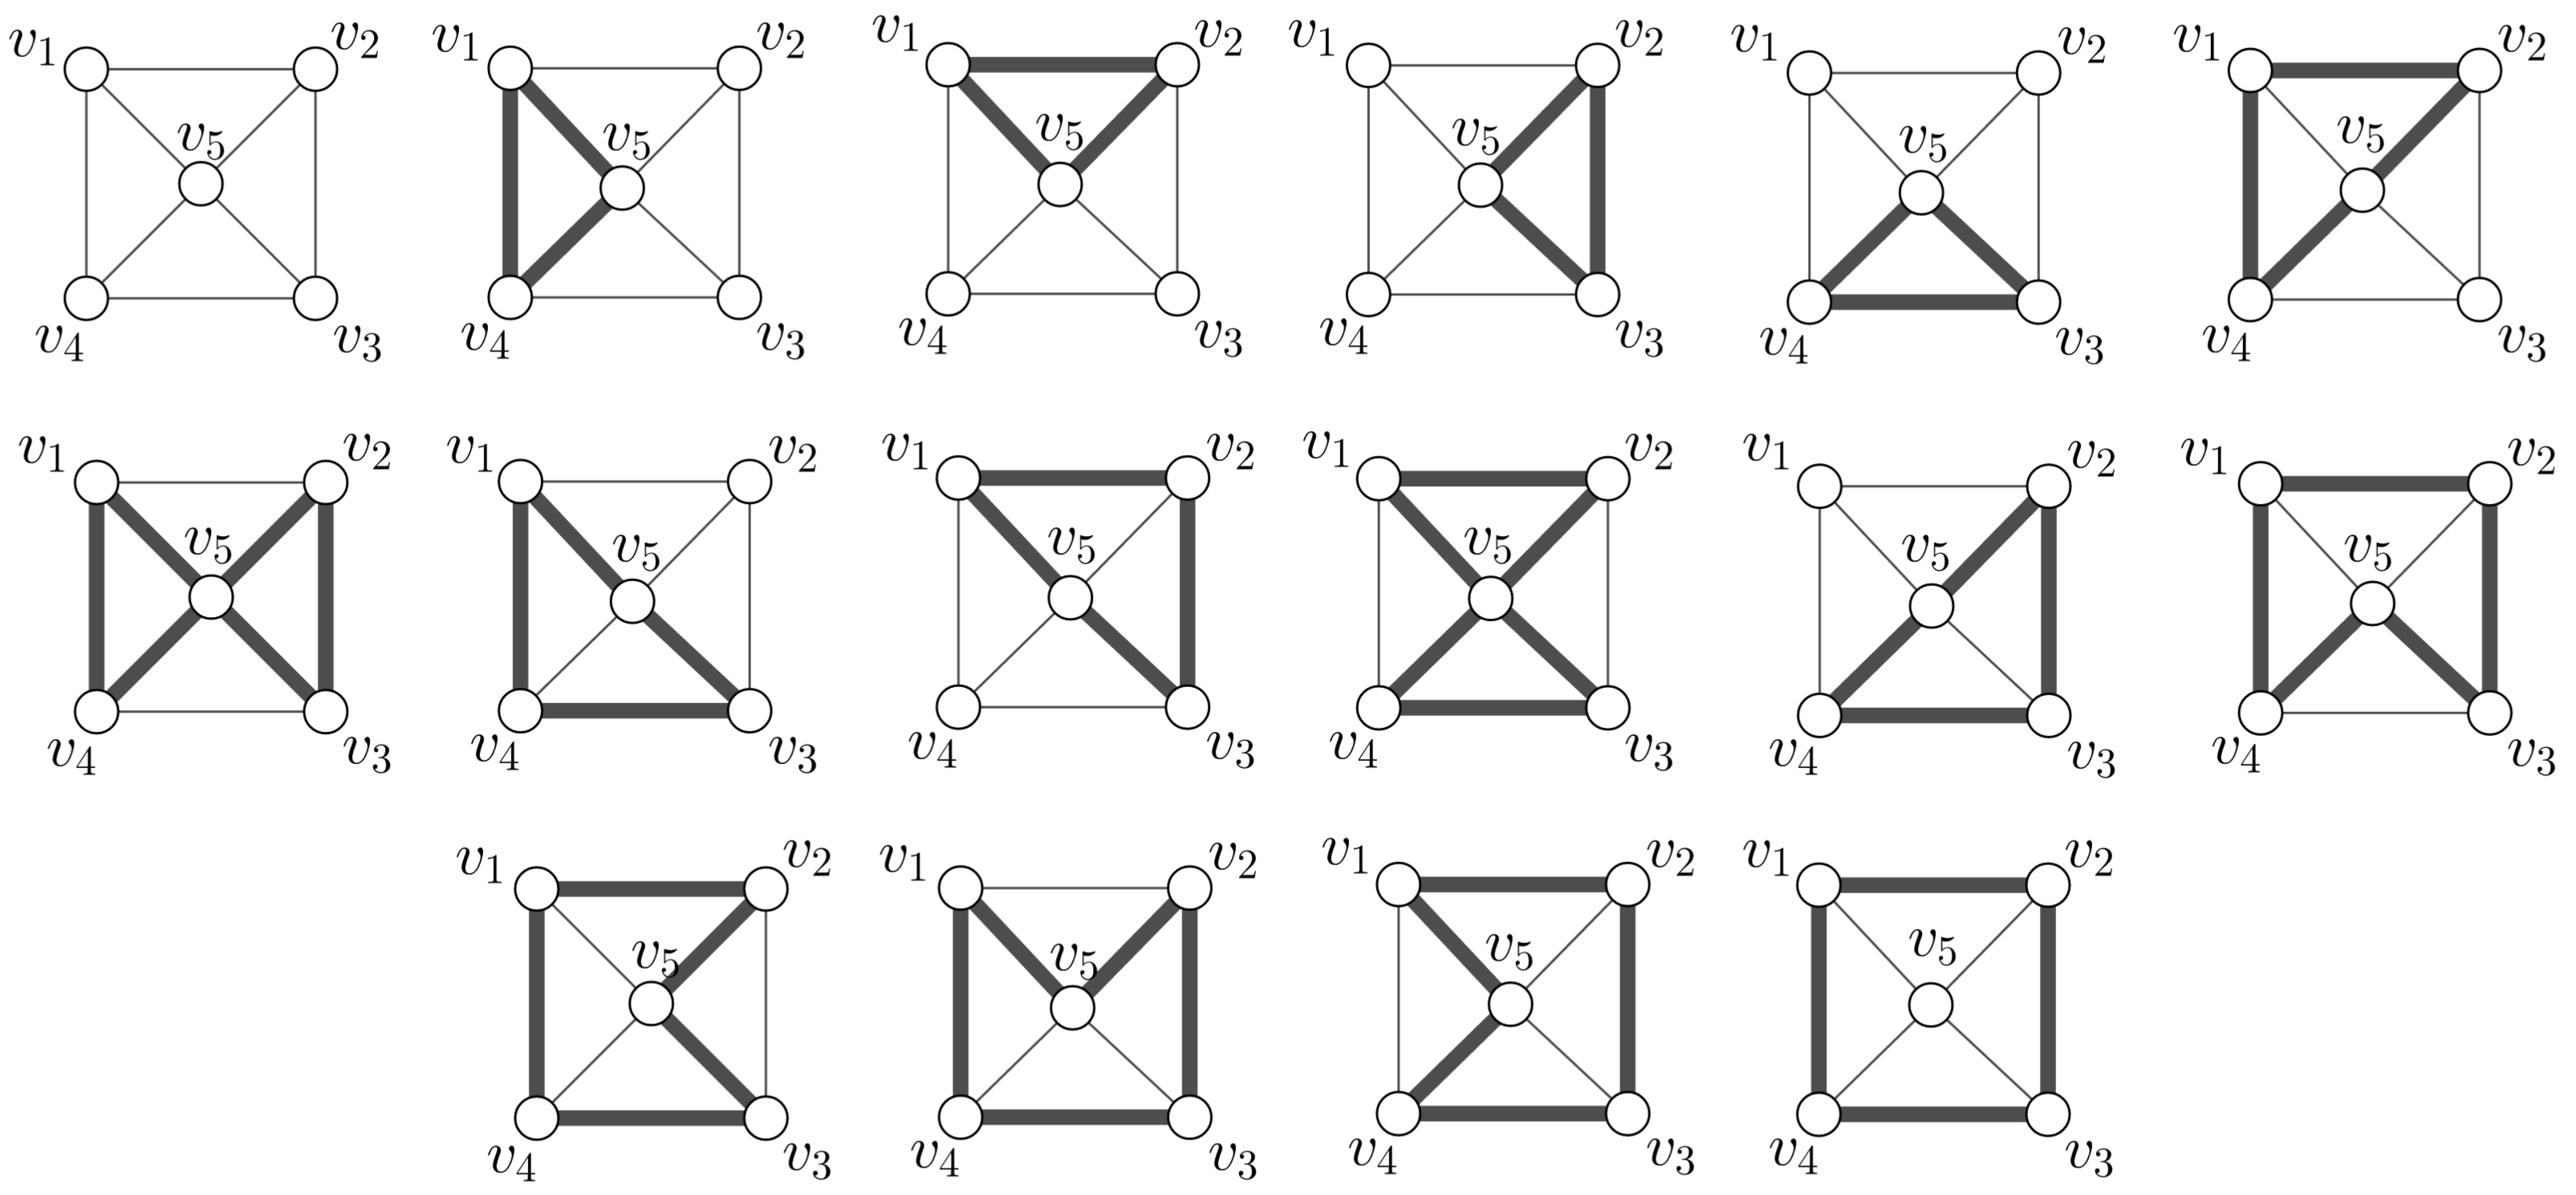
\includegraphics[width=1\textwidth]{img/imgchapter2/Espaciodeciclos.jpg}
    \caption{}
    \label{fig:espaciociclos}
\end{figure}
El lector podrá darse cuenta cómo cada subgráfica par de $W_{4}$ o es un ciclo o puede ser descompuesto en ciclos ajenos.

\hfill $\blacklozenge$
\end{ejem}

A principios del siglo XX, Oswald Veblen (1880 - 1960) caracterizó las gráficas pares como aquellas que pueden ser descompuestas en ciclos ajenos. Una \textit{descomposición} de una gráfica $G$ es una familia $\mathcal{F}$ de subgráficas ajenas por aristas tales que:
$$
\bigcup_{F \in \mathcal{F}} E(F) = E(G).
$$

A continuación presentamos dicho resultado y su justificación. Cabe aclarar que cuando decimos \textit{ciclos ajenos} nos referimos a ciclos \textit{ajenos por aristas}. 

\begin{teo}[\textit{\textbf{Teorema de Veblen}}] \label{teo:veblen}
Una gráfica $G$ es par si y sólo si $G$ se descompone en ciclos ajenos.
\end{teo}

\begin{proof}
Probemos la \textit{ida} por inducción fuerte, sobre el número $m$ de aristas de $G$. 

\underline{Paso base}: $m=0$. Entonces $G$ no tiene aristas, i.e., es una gráfica vacía (que es par) y se descompone en una familia vacía de ciclos.

\underline{Hipótesis de inducción}: Supongamos que, para cualquier gráfica par $H$ con $q$ aristas y $q < m$, $H$ admite una descomposición en ciclos ajenos.

\underline{Paso inductivo}: Sea $G$ una gráfica par con $m$ aristas. Tomamos $F$ la subgráfica de $G$ inducida por sus vértices de grado positivo (en otras palabras, ignoramos, de momento, los posibles vértices aislados de $G$). Dado un vértice $v \in V(F)$, por la paridad de $G$, sabemos que $d_{F}(v)\geq 2$; y, por el teorema \ref{teo:ciclos}, necesariamente $F$ contiene un ciclo, digamos $C$. Es claro también que $C$ está contenido en $G$.

Consideramos a $H = G \setminus E(C)$. Verifiquemos que esta gráfica, en efecto, es par. Tomamos $v$ un vértice cualquiera de $H$. Como $V(H) = V(G)$, $v \in V(G)$. Si es un vértice aislado, entonces su grado es par. Si no es aislado, entonces hay dos posibilidades: que $v$ sea parte del ciclo $C$ o no. Si $v \in V(C)$, significa que hay dos aristas de ese ciclo que inciden en él. Entonces, en $H$, se remueven tales aristas, disminuyendo en dos el grado de $v$ (conservando así la paridad). Si $v \notin V(C)$, su grado permanece invariante en $H$. En cualquier caso, debido a que $G$ es par, el grado de $v$ es un número par. 

Podemos resumir las ideas anteriores en la siguiente ecuación:
$$
  d_{H}(v) = \left\{\begin{matrix}
0, & \text{si} \hspace{1.5mm} d_{G}(v)=0 \\ 
d_{G}(v)-2, & \text{si} \hspace{1.5mm} v \in V(C)     \\
d_{G}(v), & \text{si} \hspace{1.5mm} v \notin V(C)
\end{matrix}\right..
$$
Por lo tanto, $H$ es una gráfica par con menos aristas que $G$. Gracias a la hipótesis de inducción sabemos que $H$ se descompone en una familia $\Gamma$ de ciclos ajenos, es decir:
$$
E(H) = \bigcup_{\gamma \in \Gamma} E(\gamma).
$$

Es sencillo notar que $C$ es un ciclo ajeno respecto a los ciclos que pertenecen a $\Gamma$. Incluso, también es cierto que 
$$
E(G) = E(H) \cup E(C) = \big( \bigcup_{\gamma \in \Gamma} E(\gamma) \big) \cup E(C). 
$$
Por consiguiente, $G$ se descompone en la familia de ciclos ajenos $\Gamma \cup \{C\}$. Por inducción, concluimos que cualquier gráfica par puede ser descompuesta en ciclos ajenos.

Probaremos ahora el \textit{regreso}. Supongamos que $G$ admite una descomposición en ciclos, i.e., que existen $\gamma_{1}, \ldots, \gamma_{q}$ ciclos ajenos contenidos en $G$ tales que 
$$
\bigcup_{i=1}^{q} E(\gamma_{i}) = E(G).
$$

Sea $v$ un vértice cualquiera de $G$. Si $v$ es aislado, o sea $d_{G}(v)=0$, entonces tiene grado par. Si $d_{G}(v)\neq 0$, significa que hay al menos otro vértice $u$ adyacente a $v$. Supongamos que $a$ es la arista cuyos extremos son $u$ y $v$. Como $a \in \bigcup_{i=1}^{q} E(\gamma_{i})$, existe un ciclo $\gamma_{j}$ tal que $a \in E(\gamma_{j})$, esto es, que $v$ es un vértice del ciclo $\gamma_{j}$, lo cual implica que existe otro vértice $w$ (éste puede ser el mismo $v$ o, incluso, $u$) adyacente a $v$. En resumen, por cada ciclo al que pertenezca $v$ otros dos vértices (no necesariamente distintos) son adyacentes a $v$, de donde $d_{\gamma_{j}}(v) = 2$. 

Por otro lado, es fácil observar que el grado de cada vértice de $G$ es la suma de los grados de ese mismo vértice respecto a cada subgráfica de la descomposición. Luego, suponiendo que $v$ es vértice de $p$ ciclos (digamos $\gamma_{j_{1}}, \ldots, \gamma_{j_{p}}$) en la descomposición, el párrafo anterior nos permite afirmar que

$$
d_{G}(v) = \sum_{i=1}^{p}d_{\gamma_{j_{i}}}(v)=\sum_{i=1}^{p}2=2p.
$$

Así, el grado de todo vértice de $G$ es el doble del número de ciclos a los que pertenece y, en consecuencia, $G$ es una gráfica par. 

Por lo tanto, $G$ es par si y sólo si $G$ se descompone en ciclos ajenos.

\end{proof}

El teorema de Veblen sugiere que los ciclos son las subgráficas pares minimales de $G$. Incluso, dicho teorema puede reformularse en términos del corolario siguiente.

\begin{cor}\label{teo:veblen2}
Una subgráfica generadora de $G$ es par si y sólo si es unión de ciclos ajenos de $G$.
 \end{cor}


\subsection{Ciclos fundamentales}
Existe un resultado similar a la proposición \ref{prop:bondintersection} para gráficas pares.

\begin{prop}
Dada cualquier subgráfica $C \neq \varnothing$ par de $G$ y cualquier árbol generador $T$, es cierto que $C \cap \overline{T} \neq \varnothing$.
\end{prop}

\begin{proof}
Si $C \cap \overline{T} = \varnothing$, entonces $C \subseteq T$. Por corolario  \ref{teo:veblen2}, $C$ se compone de ciclos de $G$. Sin embargo, esto es una contradicción pues sabemos que $T$ no contiene ciclos. Entonces $C \cap \overline{T} \neq \varnothing$.

\end{proof}

De este resultado se desprende que la única subgráfica par contenida en $T$ es la subgráfica vacía $\varnothing$, i.e., $\varnothing \subseteq T$.


Tomemos una arista $c$ cualquiera  de $\overline{T}$ y supongamos que $x$ y $y$ son sus extremos. Del teorema \ref{prop:treepath}, sabemos que hay una única trayectoria $P \subseteq T$ que une a $x$ y a $y$. Por tanto, la gráfica $T + c$ contiene al ciclo $xPycx$, llamado \textit{ciclo fundamental de} $G$ con respecto a $T$ y a $c$. Téngase en cuenta que diferentes árboles generadores determinan ciclos fundamentales distintos. Cuando esté implícito el árbol con el que estemos trabajando, escribiremos como $\mathscr{C}_{c}$ a los ciclos fundamenales con respecto a $c$. 

De forma análoga al comportamiento de los cortes fundamentales, la diferencia simétrica de dos ciclos fundamentales es una gráfica par por el teorema \ref{teo:difsimciclos}. Además, por construcción, es claro que $\mathscr{C}_{c} \cap \overline{T} = \{c\}$ y que $\mathscr{C}_{c} \subseteq T + c$. De hecho, el siguiente teorema hace uso de estas dos observaciones.

\begin{prop} \label{ciclosfundamentalespropchida}
Sea $S \subseteq \overline{T}$ una subgráfica generadora de $G$. Consideremos  
$$
C =\difsym_{c \in E(S)} \mathscr{C}_{c} 
$$
 Entonces $C$ es una subgráfica par. Además, $C \cap \overline{T} = S$ y $C$ es la única subgráfica par de $G$ con esta propiedad.
\end{prop}
 
 \begin{proof}
 Que $C$ sea par se da por el teorema \ref{teo:difsimciclos}. Por otro lado, nótese que
\begin{align*}
    C \cap \overline{T} &=(\difsym_{c \in E(S)} \mathscr{C}_{c}) \cap \overline{T} \\
             &=\difsym_{c \in E(S)} (\mathscr{C}_{c} \cap T) \\
             &=\difsym_{c\in E(S)} c \\
             &= S.
\end{align*}
Además, si hubiese otra subgráfica par $C'$ tal que $C' \cap \overline{T}= S$, entonces $(C \triangle C') \cap \overline{T} = \varnothing$. Así, $C \triangle C' \subseteq T$ y $C = C'$, y $C$ es único.
 \end{proof}

 \begin{cor} \label{cor:baseciclosfundamentales}
Todo subgráfica par de $G$ puede expresarse de manera única como una diferencia simétrica de ciclos fundamentales con respecto a $T$  
 \end{cor}
 
 \begin{proof}
 Sea $C$ una subgráfica par cualquiera de $G$. Hacemos $S= C \cap \overline{T}$. Por el teorema anterior, necesariamente, $C = \difsym_{c \in E(S)} \mathscr{C}_{c}$ y es el único con tales propiedades. 
 
 \end{proof}
 
 Sabemos que hay $m - n + 1$ aristas en $\overline{T}$. Ésto implica que $G$ debe contener $m - n +1$ ciclos fundamentales con respecto a $T$.
 
 \begin{ejem}
 Recuérdese el ejemplo \ref{ejem:cortesfundamentales} y el árbol generador $T$ que habíamos escogido para $W_{4}$ que vemos en el inciso $(a)$ de la imagen \ref{fig:ciclosfundamentales}. En el inciso $(b)$ mostramos dos ciclos fundamentales, uno respecto a la cuerda $h$ y el otro respecto a $b$.
 
 \begin{figure}[H]
     \centering
     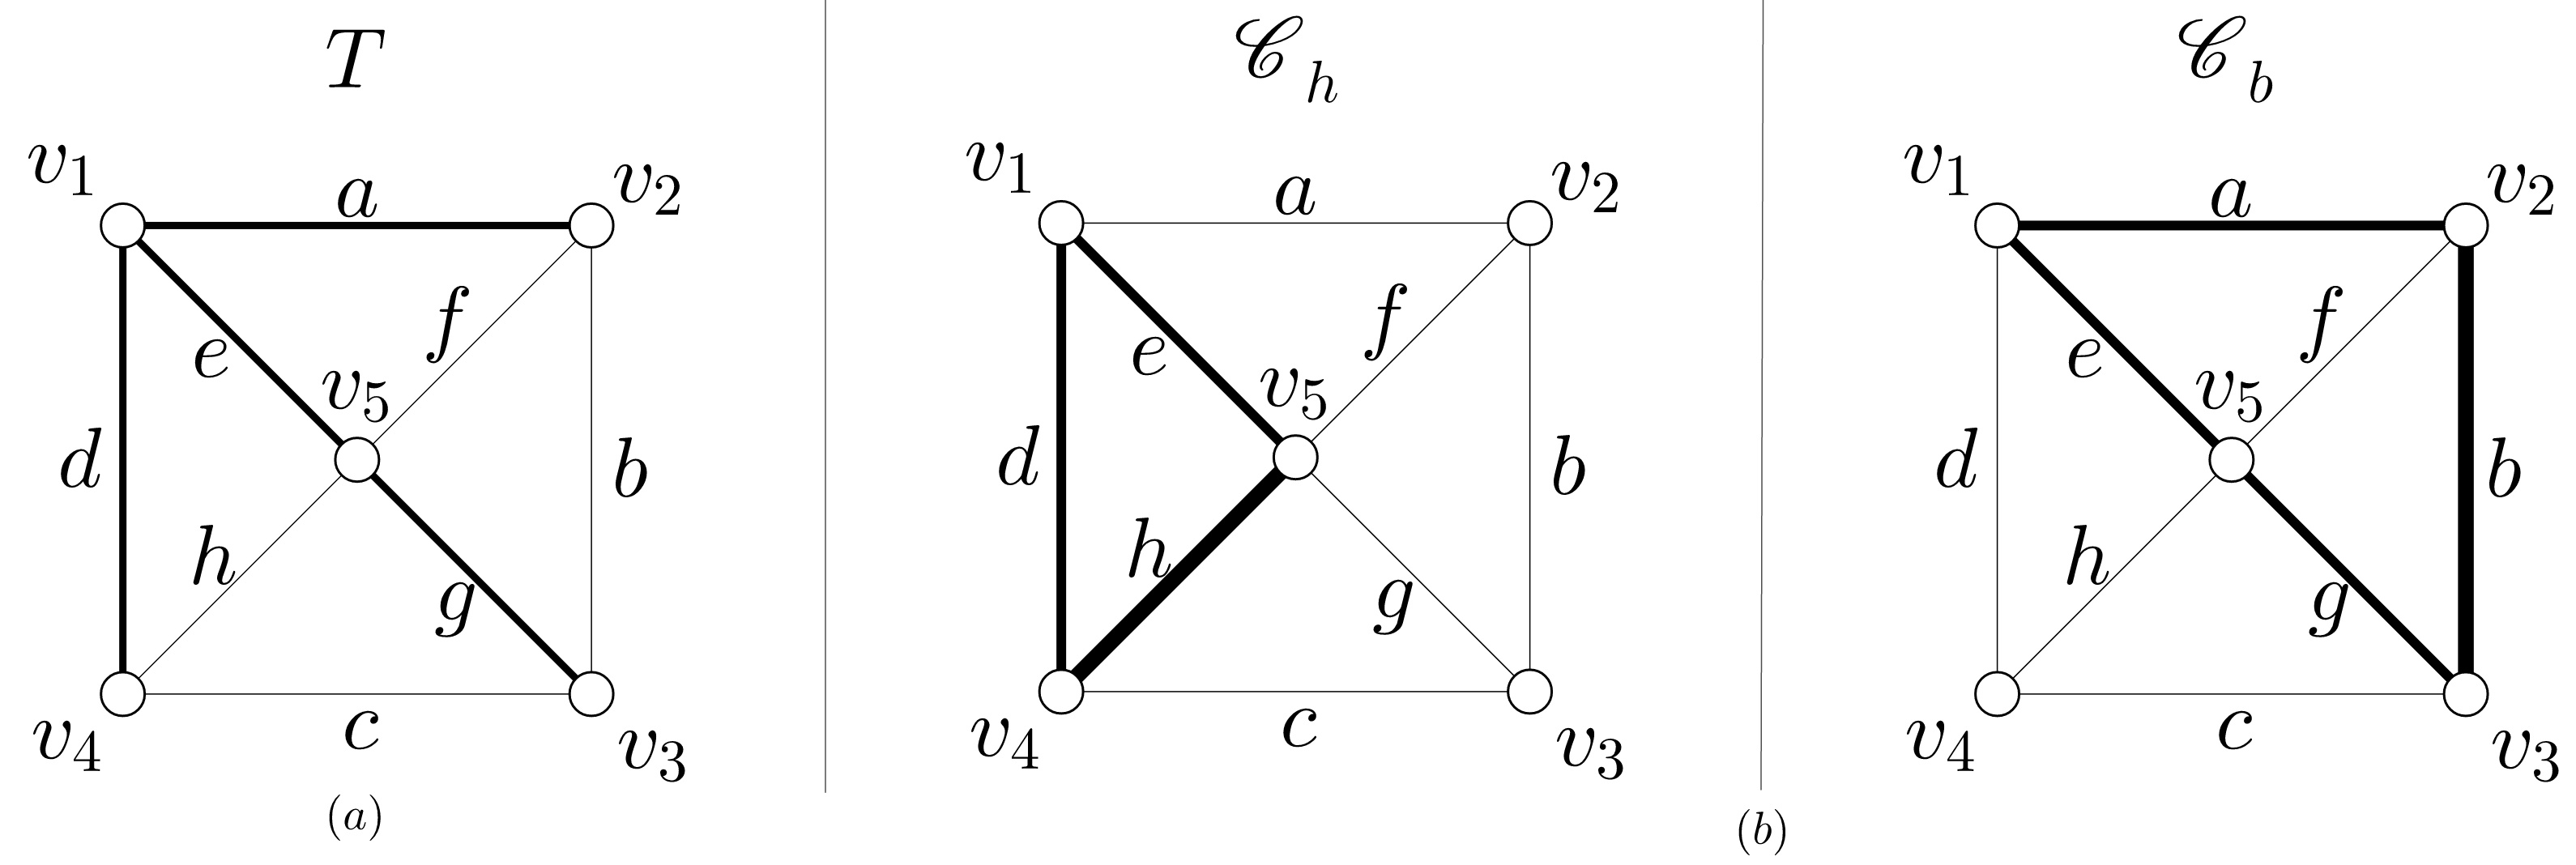
\includegraphics[scale=0.15]{img/imgchapter2/ciclosfundamentales.jpg}
     \caption{}
     \label{fig:ciclosfundamentales}
 \end{figure}
 
 \hfill $\blacklozenge$.
 \end{ejem}
 
 \section{Relación entre los conjuntos de corte y las gráficas pares}
 Tomemos un ciclo $C \subseteq g$ y un vértice $u$ de $G$. Es sencillo convencerse de que $\partial(u) \cap E(C)$ sólo tiene dos posibilidades: ser vacío o tener dos aristas como únicos elementos. En ambos casos, tal intersección es de cardinalidad par. De hecho, generalizamos estas observaciones en el siguiente teorema.

\begin{teo} \label{teo:interseccionpar}
En cualquier gráfica, toda subgráfica par y todo conjunto de corte tienen en común una cantidad par de aristas.
\end{teo}

\begin{proof}
Sea $\partial(X)$ un conjunto de corte cualquiera. Si éste es vacío, el teorema de cumple. Supongamos que $\partial(X) \neq \varnothing$.

Tomemos primero un ciclo $C$ de $G$. Si este ciclo está completamente contenido en $G[X]$ o $G[\overline{X}]$, también el teorema se cumple pues $C \cap \partial(X) = \varnothing$. La última posibilidad es que $C \cap \partial(X) \neq \varnothing$. Si ésto ocurre, significa que existe una arista con un extremo en $X$ y otro en $\overline{X}$. De tal manera que, partiendo del extremo en $X$, el ciclo atraviesa la gráfica hasta regresar al vértice donde empezó. Entonces $C$ cruza de $X$ a $\overline{X}$ las mismas veces que cruza de $\overline{X}$ a $X$. Por tanto, $|C \cap \partial(X)|$ es un número par en los casos posibles.

Gracias al teorema \ref{teo:veblen2} y al párrafo anterior, podemos asegurar la veracidad del teorema.

\end{proof}

 \begin{figure}[t]
     \centering
     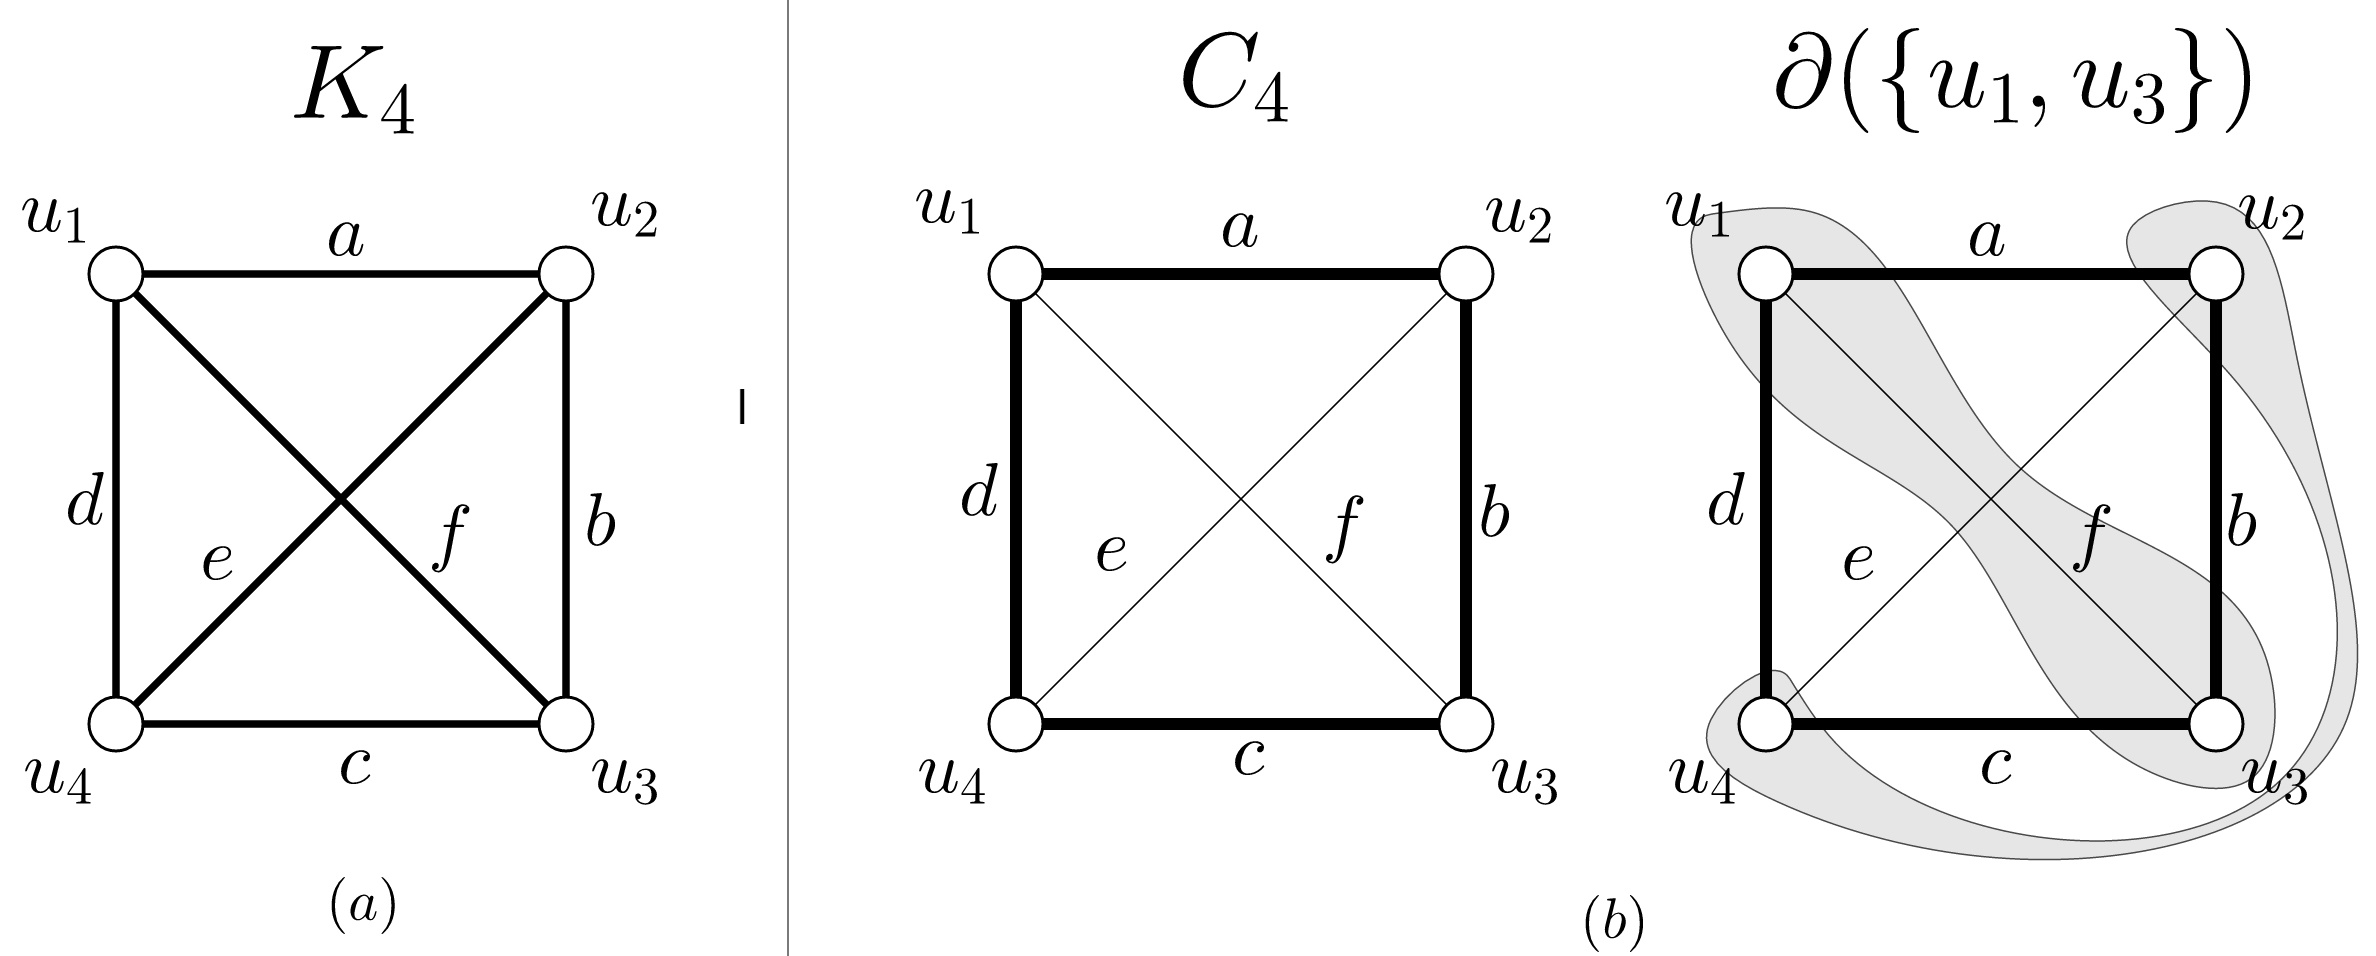
\includegraphics[scale=0.2]{img/imgchapter2/k4ciclocorte.jpg}
     \caption{}
     \label{fig:k4ciclocorte}
 \end{figure}
¿Hay conjuntos de corte que son gráficas pares también? ¿O son conceptos mutuamente excluyentes? La respuesta es afirmativa: hay gráficas pares que, al mismo tiempo, son conjuntos de corte, como vemos en el siguiente ejemplo.

\begin{ejem} \label{ejem:k4ciclocorte}
Consideremos a $K_{4}$, la gráfica completa de cuatro vértices (inciso $(a)$ de la figura \ref{fig:k4ciclocorte}). Es evidente que contiene al ciclo $C_{4}$, cuyas aristas son $\{a,b,c,d\}$. Si observamos atentamente, uno puede darse cuenta que $\partial{\{u_{1},u_{3}\}} = C_{4}$.

 \hfill $\blacklozenge$
\end{ejem}
 
 
 \section{¿Y si $G$ es inconexa?}
 Estudiemos ahora qué comportamiento tienen los cortes y los ciclos en las gráficas inconexas. Supongamos que $G$ tiene $c:=c(G)$ componentes conexas y que éstas son $F_{1}, \ldots, F_{c}$\footnote{Tómese en cuenta que, en nuestro contexto, cada componente conexa la estamos viendo como una subgráfica generadora de $G$}, i.e., 
$$
G = \bigcup_{i=1}^{c}F_{i}.
$$
  \subsection{Conjuntos de corte}
   Tomemos $X \subseteq V(G) = \cup_{i = 1}^{c}V(F_{i})$. Puesto que no hay aristas que conecten vértices de diferentes componente conexas, necesariamente $$\partial_{G}(X) = \bigcup_{i=1}^{c} \partial_{F_{i}}(X_{i}),$$ con $X_{i}:=X \cap V(F_{i})$, $\partial_{F_{i}}(X_{i})\subseteq G$ e $i \in \{1, \ldots, c\}$.
   
   Lo anterior implica que los conjuntos de corte minimales de $G$ son los cortes minimales de cada componente $F_{i}$ (como subgráficas generadoras de $G$). De antemano, es claro que $\partial_{G}(X)$ divide a $G$ en, al menos, $c+1$ componentes. Pero, en virtud del teorema \ref{teo:caracterizacionbond}, si $\partial_{G}(X):=\partial_{F_{j}}(X_{j})$ es un corte minimal, entonces $G\setminus \partial_{G}(X)$ tiene, exactamente, $c+1$ componentes conexas. El recíproco es también cierto y ésta es una generalización del mencionado teorema \ref{teo:caracterizacionbond} que dejaremos establecida en el siguiente enunciado.
   
   \textcolor{red}{QUITAR "DE ANTEMANO". QUITAR COMAS EN "AL MENOS", AGREGAR PREGUNTAR ¿CUÁNDO SE ALCANZA LA IGUALDAD? IDA RIGUROSA
   
   Para la suficiencia explicar caso c=1
   
   Caso c=2, "se tiene" "continuando con este procedimiento"
   
   qui}
   
   \begin{teo} \label{teo:caracterizacionbond2}
   $\partial(X)$ es un corte minimal si y sólo si $c(G\setminus \partial(X)) = c(G) + 1$
   \end{teo}
   \begin{proof} Ya discutimos que la \textit{necesidad} se debe al teorema \ref{teo:caracterizacionbond}.
   
   Para la \textit{suficiencia}  asumimos que $G \setminus \partial(X)$ tiene $c+1$ componentes conexas. Si $c=1$, se sigue del recíproco del multicitado teorema \ref{teo:caracterizacionbond}. Pensemos ahora que $c\geq 2$ y supogamos primero que, para cada $i \in \{1, \ldots, c\}$, $X_{i} \neq \emptyset$ (ver la figura \ref{fig:componentes}). Por tanto, ya sabemos que
$$\partial(X)=\bigcup_{i=1}^{c}\partial_{F_{i}}(X_{i}).$$
De tal forma que $G \setminus \partial(X)=\bigcup_{i=1}^{c}(F_{i} \setminus \partial_{F_{i}}(X_{i}))$. Dado que $\partial_{F_{i}}(X_{i})$ es un conjunto de corte de $F_{i}$, entonces $F_{i} \setminus \partial_{F_{i}}(X_{i})$ posee, al menos, dos componentes conexas, para cada $i \in \{1, \ldots, c\}$. Luego, $G \setminus \partial(X)$ tiene, al menos, $2c$ componentes. Sin embargo, esto no es posible pues, por hipótesis, hay sólo $c+1$ componentes conexas y $2c = c+1$ si y sólo si $c=1$. La contradicción vino de suponer que los conjuntos $X_{i}$ son no vacíos. Entonces existe algún $X_{j} = \emptyset$. 

\begin{figure}[H]
    \centering
    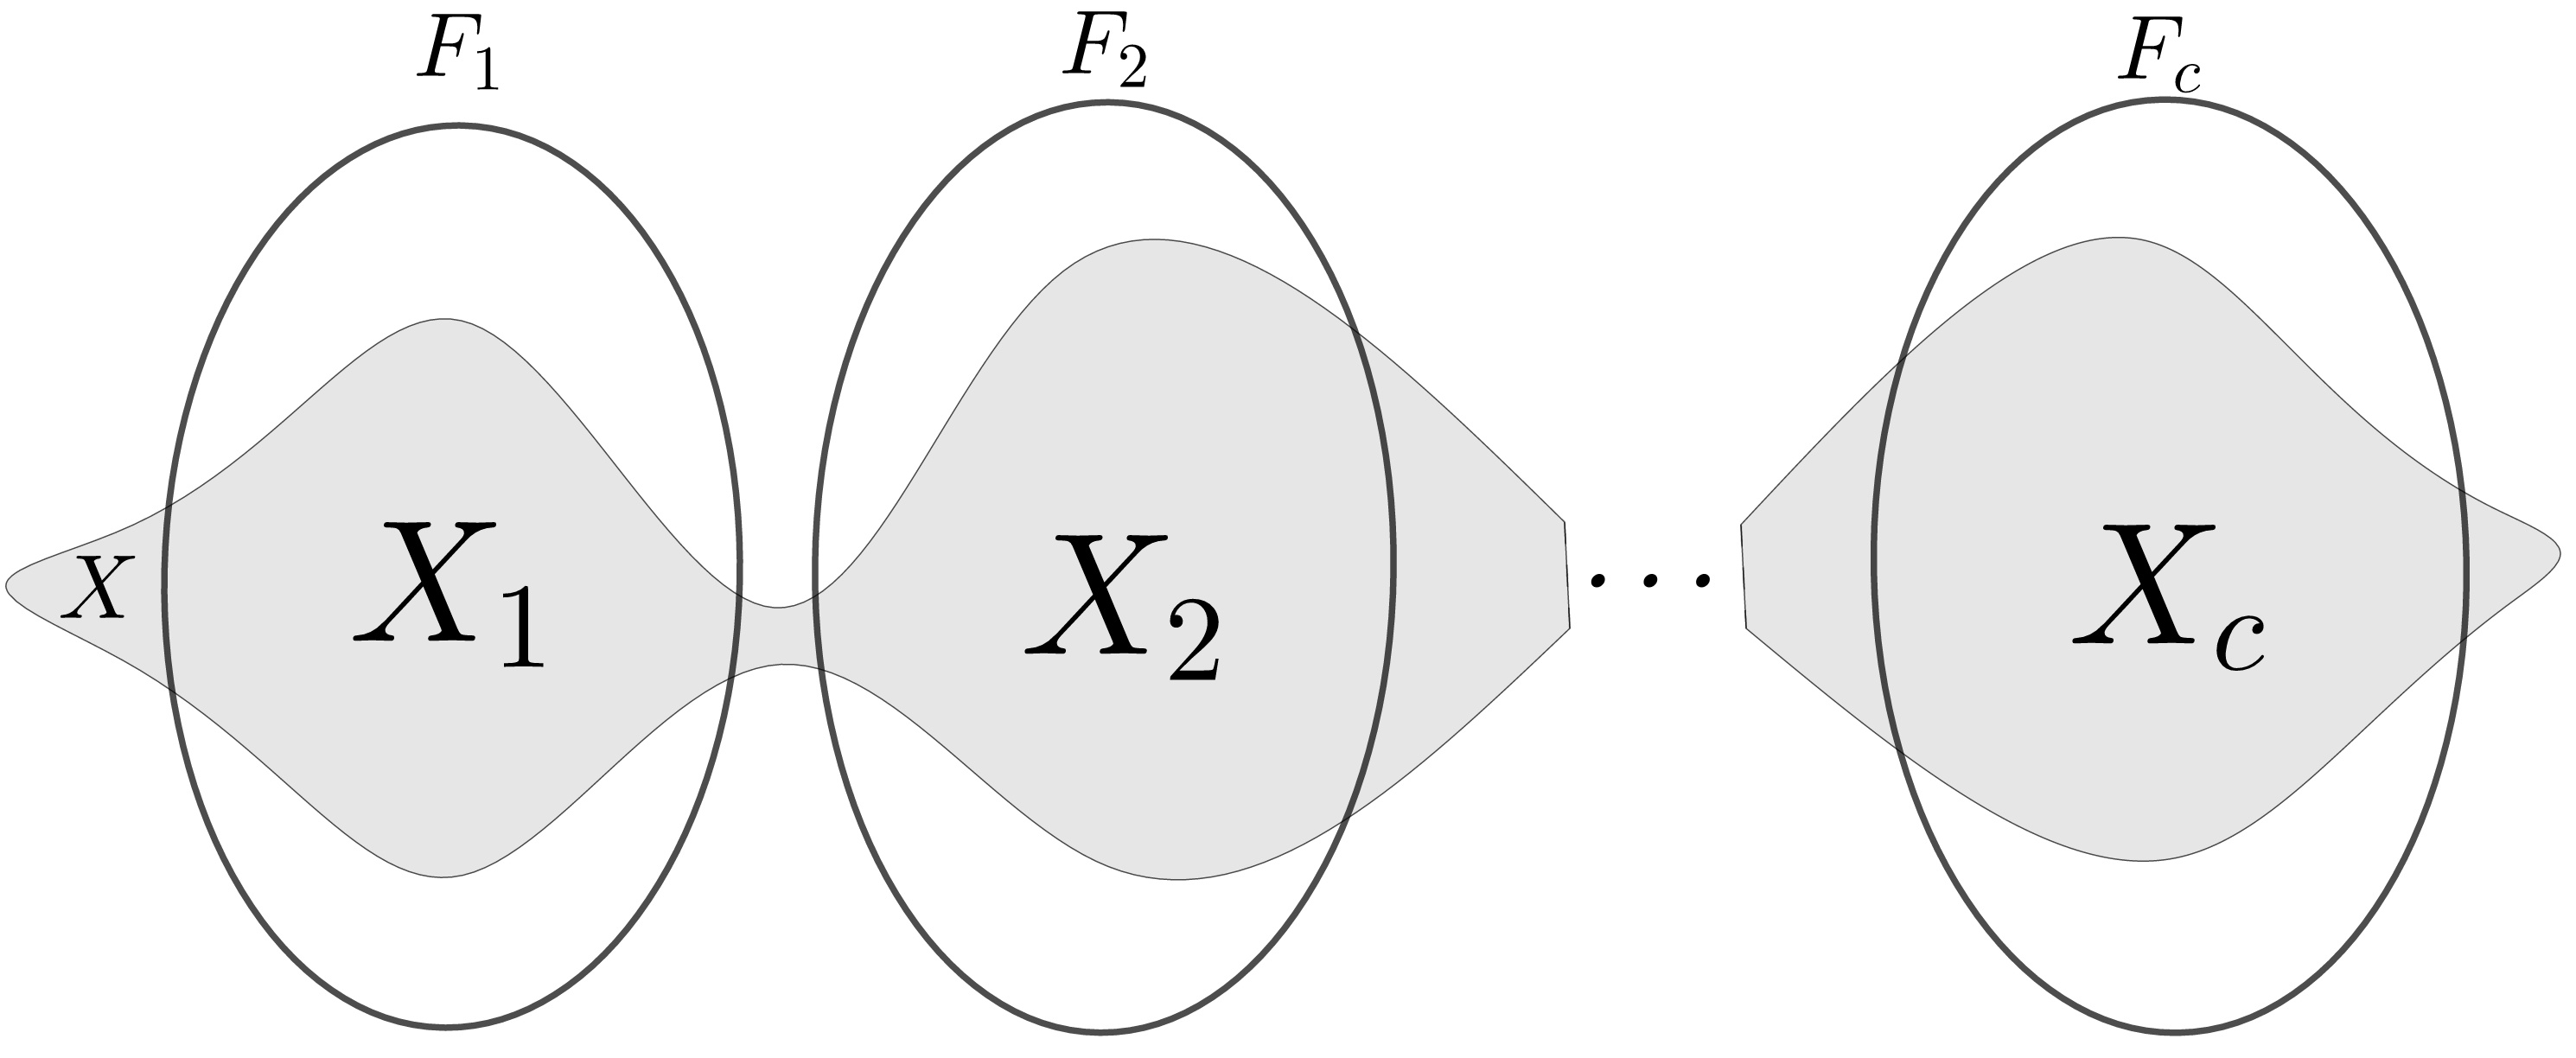
\includegraphics[scale=0.15]{img/imgchapter2/componentes.jpg}
    \caption{}
    \label{fig:componentes}
\end{figure}

Sin pérdida de generalidad, digamos que $X_{c}:=X_{j}$. Así, $$\partial(X) = \bigcup_{i=1}^{c-1} \partial_{F_{i}}(X_{i})$$. Suponiendo las hipótesis y siguiendo el mismo razonamiento del párrafo anterior, obtenemos que $G\setminus \partial(X)$ tiene\footnote{Añadimos un ``$1$'' porque contamos la componente $F_{c}$.}, al menos, $2(c-1) + 1$. Dado que $G \setminus \partial(X)$ tiene $c+1$ componentes conexas, entonces $2(c-1) + 1 \geq c+1$. 

Si $c=2$, terminamos pues se tendría $2(c-1)+1 = c+1$ y $\partial(X) = \bigcup_{i=1}^{c-1} \partial_{F_{i}}(X_{i})= \partial_{F_{1}}(X_{1})$. Si $c \geq 2$, entonces $2(c-1) + 1 > c+1$, una contradicción. Así, hay algún $X_{j} =\emptyset$, digamos $X_{c-1}:=X_{j}$. Continuando con estos argumentos, eventualmente llegaremos a que $\partial(X) = \partial_{F_{1}}(X_{1})$. Como tampoco los $X_{i}$ pueden ser todos vacíos a la vez porque $\partial(X) \neq \emptyset$, deducimos que $X_{1} \neq \emptyset$. 


Por consiguiente, y del hecho de que hay exactamente $c+1$ componentes, se desprende que $X_{1}$ cumple tres cosas: que $X_{1} \neq \emptyset$, que $F_{1} \setminus \partial_{F_{1}}(X_{1})$ tiene exactamente dos componentes conexas y que $\partial_{F_{1}}(X_{1})=\partial(X)$. En otras palabras, $\partial_{F_{1}}(X_{1})$ es un conjunto de corte minimal de $F_{1})$ igual a $\partial(X)$. Como los conjuntos de corte minimales de cada componente conexa lo son también de $G$, obtenemos que $\partial(X)$ es un conjunto de corte minimal de $G$.

En conclusión, $\partial(X)$ es un conjunto de corte minimal si y sólo si $G \setminus \partial(X)$ tiene exactamente $c+1$ componentes conexas.

\end{proof}
   
   Además de que el teorema \ref{teo:unionajenademinimales} sigue siendo válido, los cortes fundamentales de $G$ son los cortes fundamentales de cada componente conexa, respecto a un bosque generador maximal. Como estos bosques tienen $n-c$ aristas, entonces $G$ tiene $n - c$ conjuntos de corte fundamentales. Los teoremas que involucran cortes fundamentales continúan siendo válidos.
 
  \subsection{Gráficas pares}
  
  Al igual que los conjuntos de corte en gráficas inconexas, los subgráficas pares de $G$ están compuestas por las subgráficas pares (consideradas como subgráficas generadoras de $G$) de cada componente conexa  $F_{i}$. Los ciclos de $G$ son los ciclos de $F_{i}$ y el teorema de Veblen se mantiene. 
  
  Los ciclos fundamentales con respecto a algún bosque generador maximal de $G$ son los ciclos fundamentales de cada componente conexa $F_{i}$. Los teoremas concernientes a éstos se mantienen. 
  
  Por último, puesto que hay $m - n + c$ cuerdas respecto a cualquier bosque generador maximal, necesariamente $G$ tiene $m-n+c$ ciclos fundamentales.
 
 \section{Cortes y ciclos en digráficas}
 La teoría de digráficas tiene una amplia literatura, como puede constatarse en \cite{Bang-Jensen}. Sin embargo en esta tesis realmente lo que nos interesa son las gráficas subyacentes de las digráficas. Concretamente, nos enfocaremos en sus cortes y sus gráficas pares y, desde luego, en los elementos mínimales de estas clases de subgráficas. Por estas razones, sólo introducimos los conceptos necesarios para tal propósito.
 
 Las digráficas son de interés pues, como se verá en el próximo capítulo, permiten asociarles espacios vectoriales sobre los reales, cosa que no sería posible si no tuvieran dirección las aristas. 
 
 A lo largo de esta sección vamos a suponer que $D = (V,A)$ es una digráfica conexa. De igual modo, consideraremos que los vértices y los arcos de $D$ ya tienen un orden, es decir, que $V(D)=\{u_{1}, \ldots, u_{n}\}$ y que $A(D)= \{ a_{1} \ldots a_{m}\}$.


 \subsection{Conjuntos de corte de $D$}
 \begin{figure}[h]
    \centering
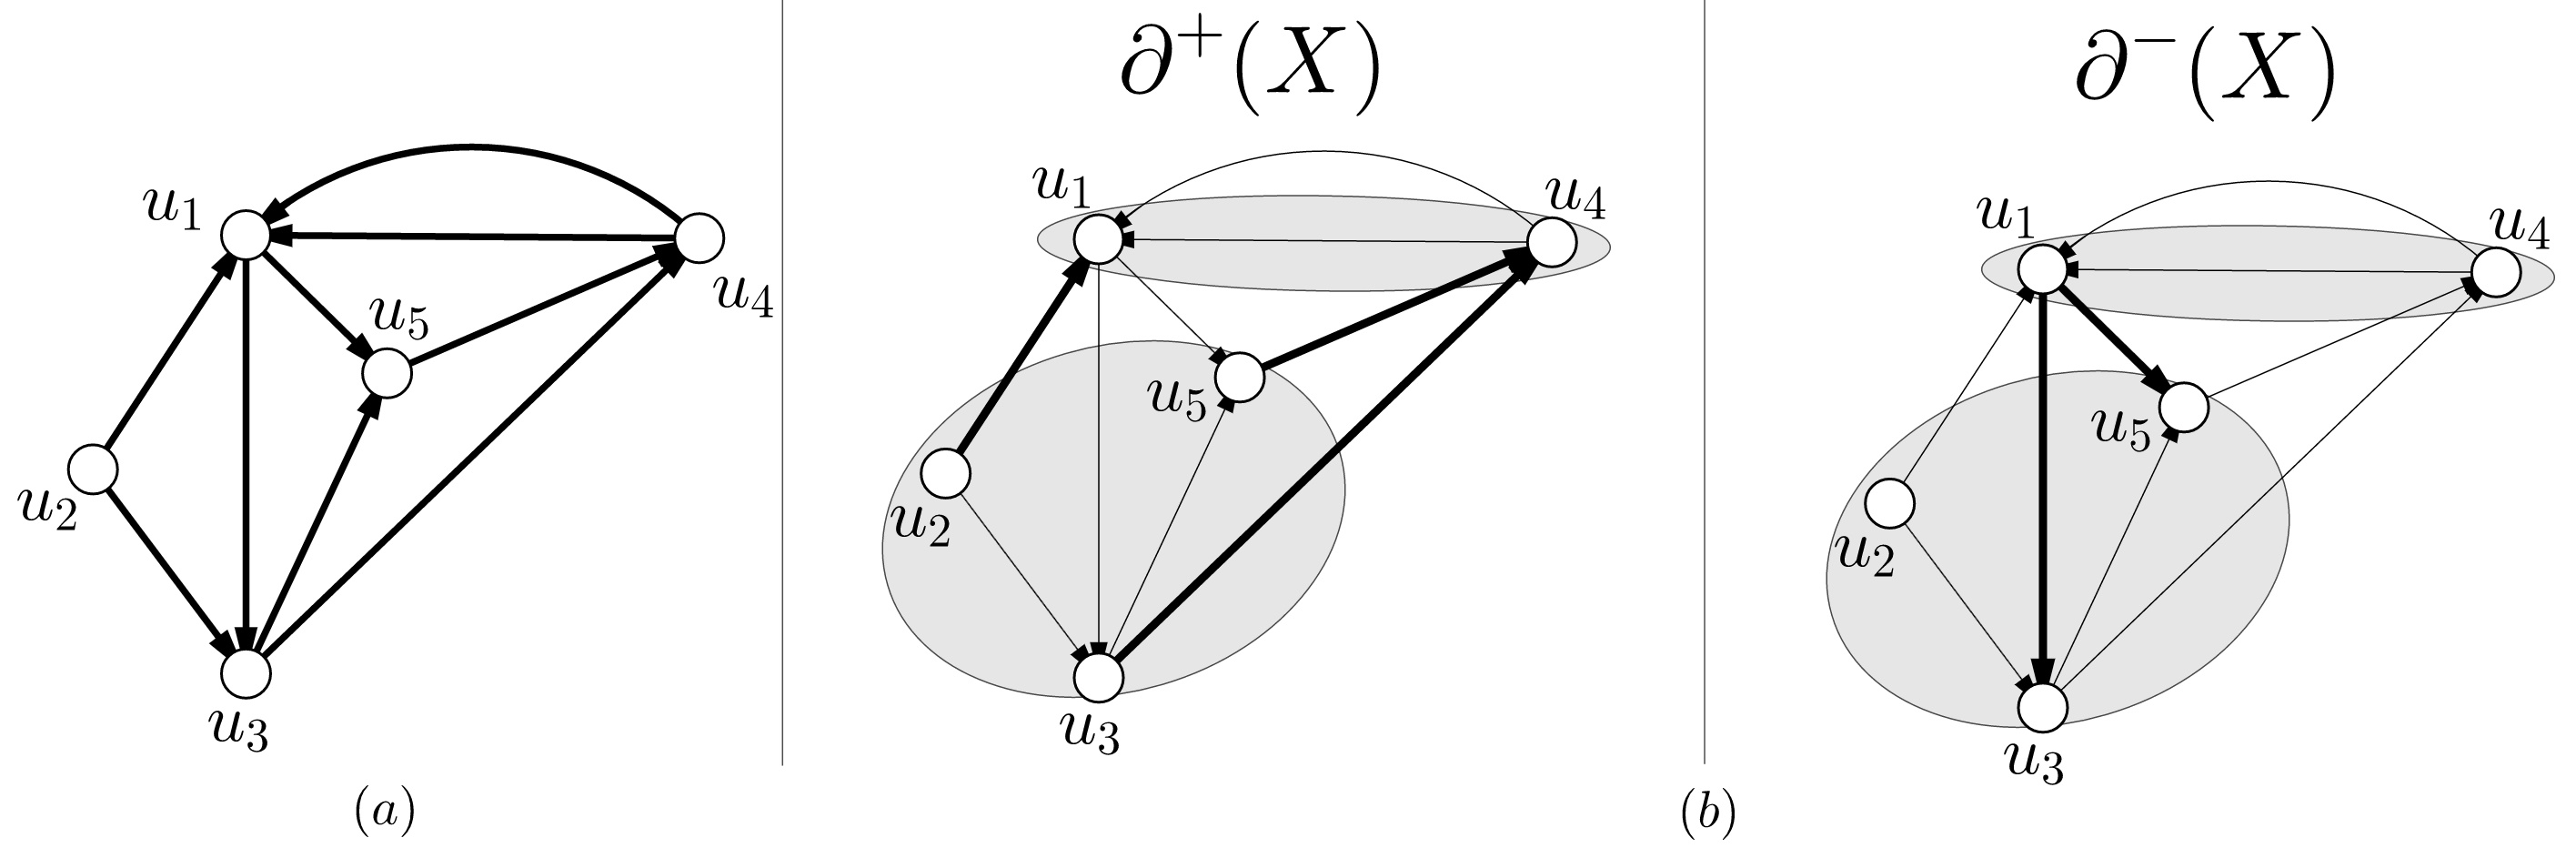
\includegraphics[scale=0.18]{img/imgchapter2/ExcorteIncorte.jpg}
    \caption{}
    \label{fig:excorteincorte}
\end{figure}
 
 Sean $X \subseteq V$ y $Y \subseteq V$. Al conjunto de arcos cuyas colas estén $X$ y cabezas en $Y$ se le denota como $A[X,Y]$. Si $Y = \overline{X}$, $\partial^{+} (X) := A[X,\overline{X}]$ es el \textit{excorte} de $D$ asociado a $X$. Similarmente, el \textit{incorte} asociado a $X$ es el conjunto $\partial^{-}(X) := A[X,\overline{X}]$. Finalmente el \textit{conjunto de corte de $D$ asociado a $X$} es la unión del excorte y el incorte respectivo, es decir, $\partial(X) := \partial^{+}(X) \cup \partial^{-}(X)$. Es sencillo observar que $\partial^{+}(X) = \partial^{-}(\overline{X})$. En la figura \ref{fig:excorteincorte} mostramos un excorte y un incorte de la digráfica del inciso $(a)$, con $X=\{u_{2},u_{3},u_{5}\}$.

Un uso de esta nueva notación es la de reescribir la definición de conexidad fuerte que dimos en un principio. En efecto, $D$ es \textit{fuertemente conexa} si y sólo si, para todo $X \subseteq V(D)$, $\partial^{+}(X) \neq \emptyset$. 

Asimismo, recordando la definición de la matriz de incidencia $\mathbf{M}_{D} = [m_{va}]$, podemos ahora establecer que:
\begin{equation} \label{eq:mva}
  m_{va}=
    \begin{cases}
\hspace{0.7em} 1, & a \in \partial^{+}(v)\\ 
-1, & a \in \partial^{-}(v)\\ 
\hspace{0.7em} 0, & \text{en otro caso}
\end{cases}
\end{equation}
Si $G:=G(D)$ es la gráfica subyacente de $D$, observe también que los elementos $\partial_{G}(X)$ son los mismos que en $\partial_{D}(X)$ pero sin considerar direcciones. De aquí que un conjunto de aristas es un corte en $G$ si y sólo si el correspondiente conjunto de arcos es un corte en $D$.

\begin{figure}[h]
    \centering
    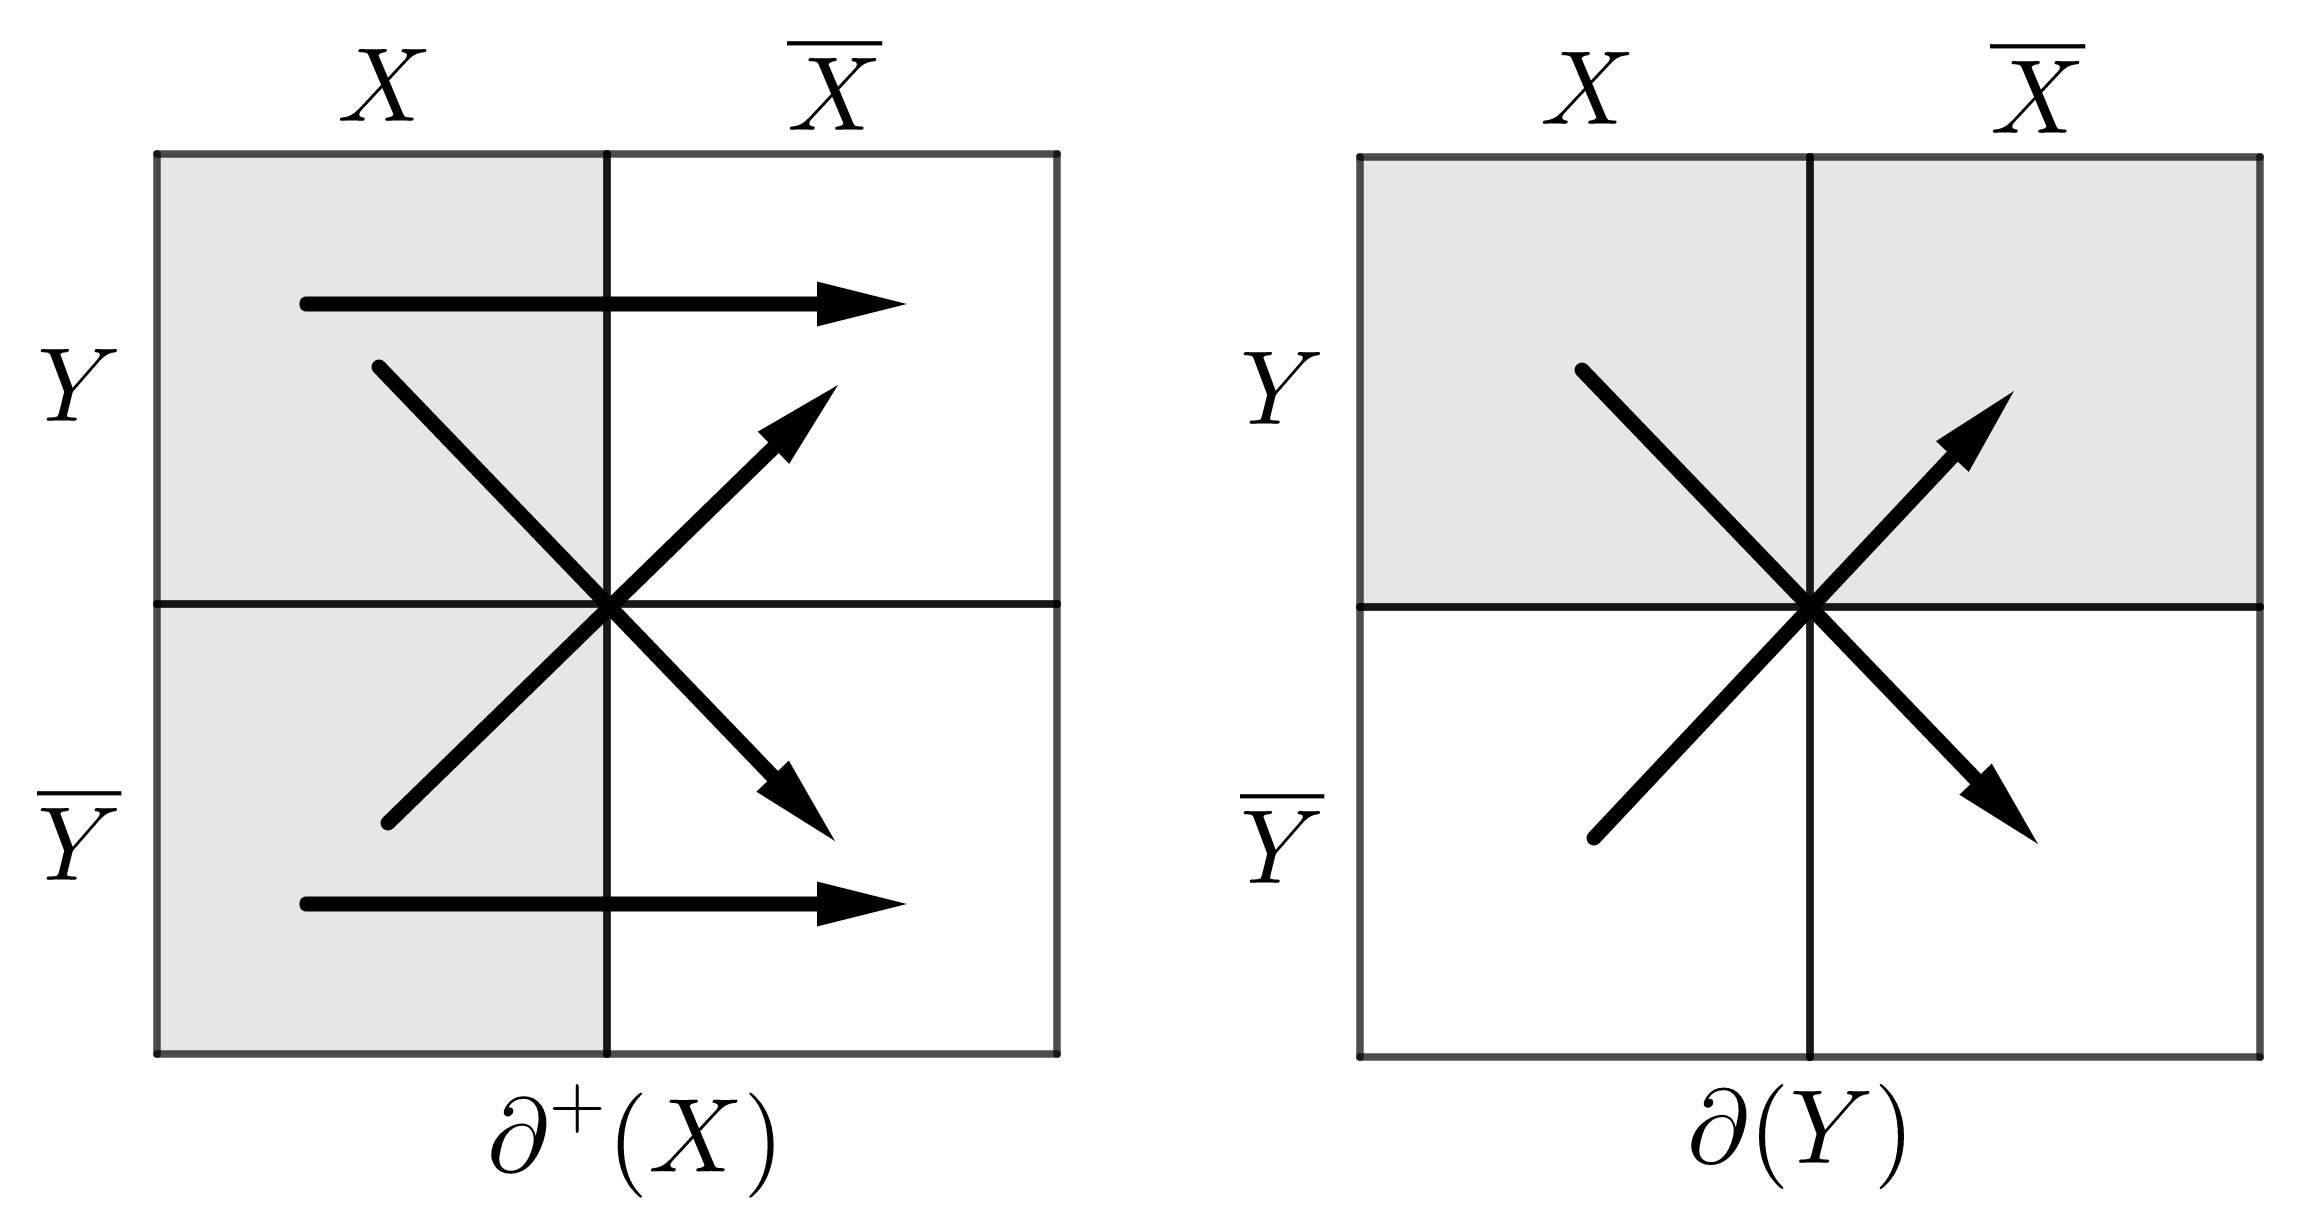
\includegraphics[scale=0.15]{img/imgchapter2/bondsdirigidos.jpg}
    \caption{}
    \label{fig:bondsdirigidos}
\end{figure}

Lo anterior nos abre paso para definir cortes minimales en digráficas. Así, un conjunto de corte $\partial_{D}(X)$ es \textit{minimal} en $D$ si y sólo si $\partial_{G}(X)$ es un corte minimal en $G$. También diremos que un conjunto de corte es \textit{dirigido} si $\partial(X) = \partial^{+}(X)$, o sea, $\partial^{-}(X)=\emptyset$.

Observemos que en cualquier corte dirigido, los cortes minimales que contiene también deben ser dirigidos. Apoyémonos de la figura \ref{fig:bondsdirigidos}. Si $\partial(X) = \partial^{+}(X)$, cualquier $\partial(Y) \subseteq \partial^{+}(X)$ es de la forma $\partial(Y) = A[X \cap Y, \overline{X} \cap \overline{Y}] \cup A[X \cap \overline{Y}, \overline{X} \cap Y] $. Sin embargo, si $\partial(Y)$ es minimal, vimos en el capítulo anterior que podemos tomar  $Y$ de tal manera que $X \cap\overline{Y} = \emptyset$. Entonces $\partial(Y)= A[X \cap Y, \overline{X} \cap \overline{Y}] = \partial^{+}(Y)$. Por lo que todo corte minimal contenido en un corte dirigido debe ser, a su vez, dirigido.


 \subsection{Los ciclos de $D$}
 
Sea $C$ un ciclo con vértices $V=\{u_{1}, \ldots, u_{n}\}$ y arcos $A=\{a_{1},\ldots, a_{n}\}$. Dependiendo fuertemente del diagrama con el que representemos al ciclo, es sencillo convencerse que puede ser \textit{recorrido} o \textit{atravesado} en dos sentidos: a favor de las manecillas del reloj (representado con el símbolo $\mathbf{\circlearrowright}$) o en contra de las manecillas del rejol (cuyo símbolo asociado es $\mathbf{\circlearrowleft})$. Dicho formalmente, en esencia, podemos asociar a $C$ dos posibles circuitos distintos: $\Gamma_{\mathbf{\circlearrowright}}=u_{1}a_{1}u_{2}\ldots u_{n}a_{n}u_{1}$ y $\Gamma_{\mathbf{\circlearrowleft}}=u_{1}a_{n}u_{n}\ldots u_{2}a_{1}u_{1}$, suponiendo que los vértices y arcos han sido ordenados y etiquetados \textit{adecuadamente}.

Como se ha visto, no necesariamente $u_{i-1}$ domina a $u_{i}$ (en $\Gamma_{\mathbf{\circlearrowright}}$), ni tampoco siempre se cumple que  $u_{i}$ domina a $u_{i-1}$ (en $\Gamma_{\mathbf{\circlearrowleft}}$). Los arcos $a_{i}$ de $\Gamma_{\mathbf{\circlearrowright}}$ para los cuales sí se da que $t(a_{i}) = u_{i-1}$ y $h(a_{i})=u_{i}$ se llaman \textit{arcos hacia adelante}\footnote{\textit{Forward arcs}, en inglés.}; y aquellos tales que $t(a_{i})=u_{i}$ y $h(a_{i})=u_{i-1}$ son \textit{arcos hacia atrás} \footnote{\textit{Reverse arcs}, en inglés}. Los arcos hacia adelante y atrás de $\Gamma_{\mathbf{\circlearrowleft}}$ son definidos análogamente.

\begin{figure}[H]
    \centering
    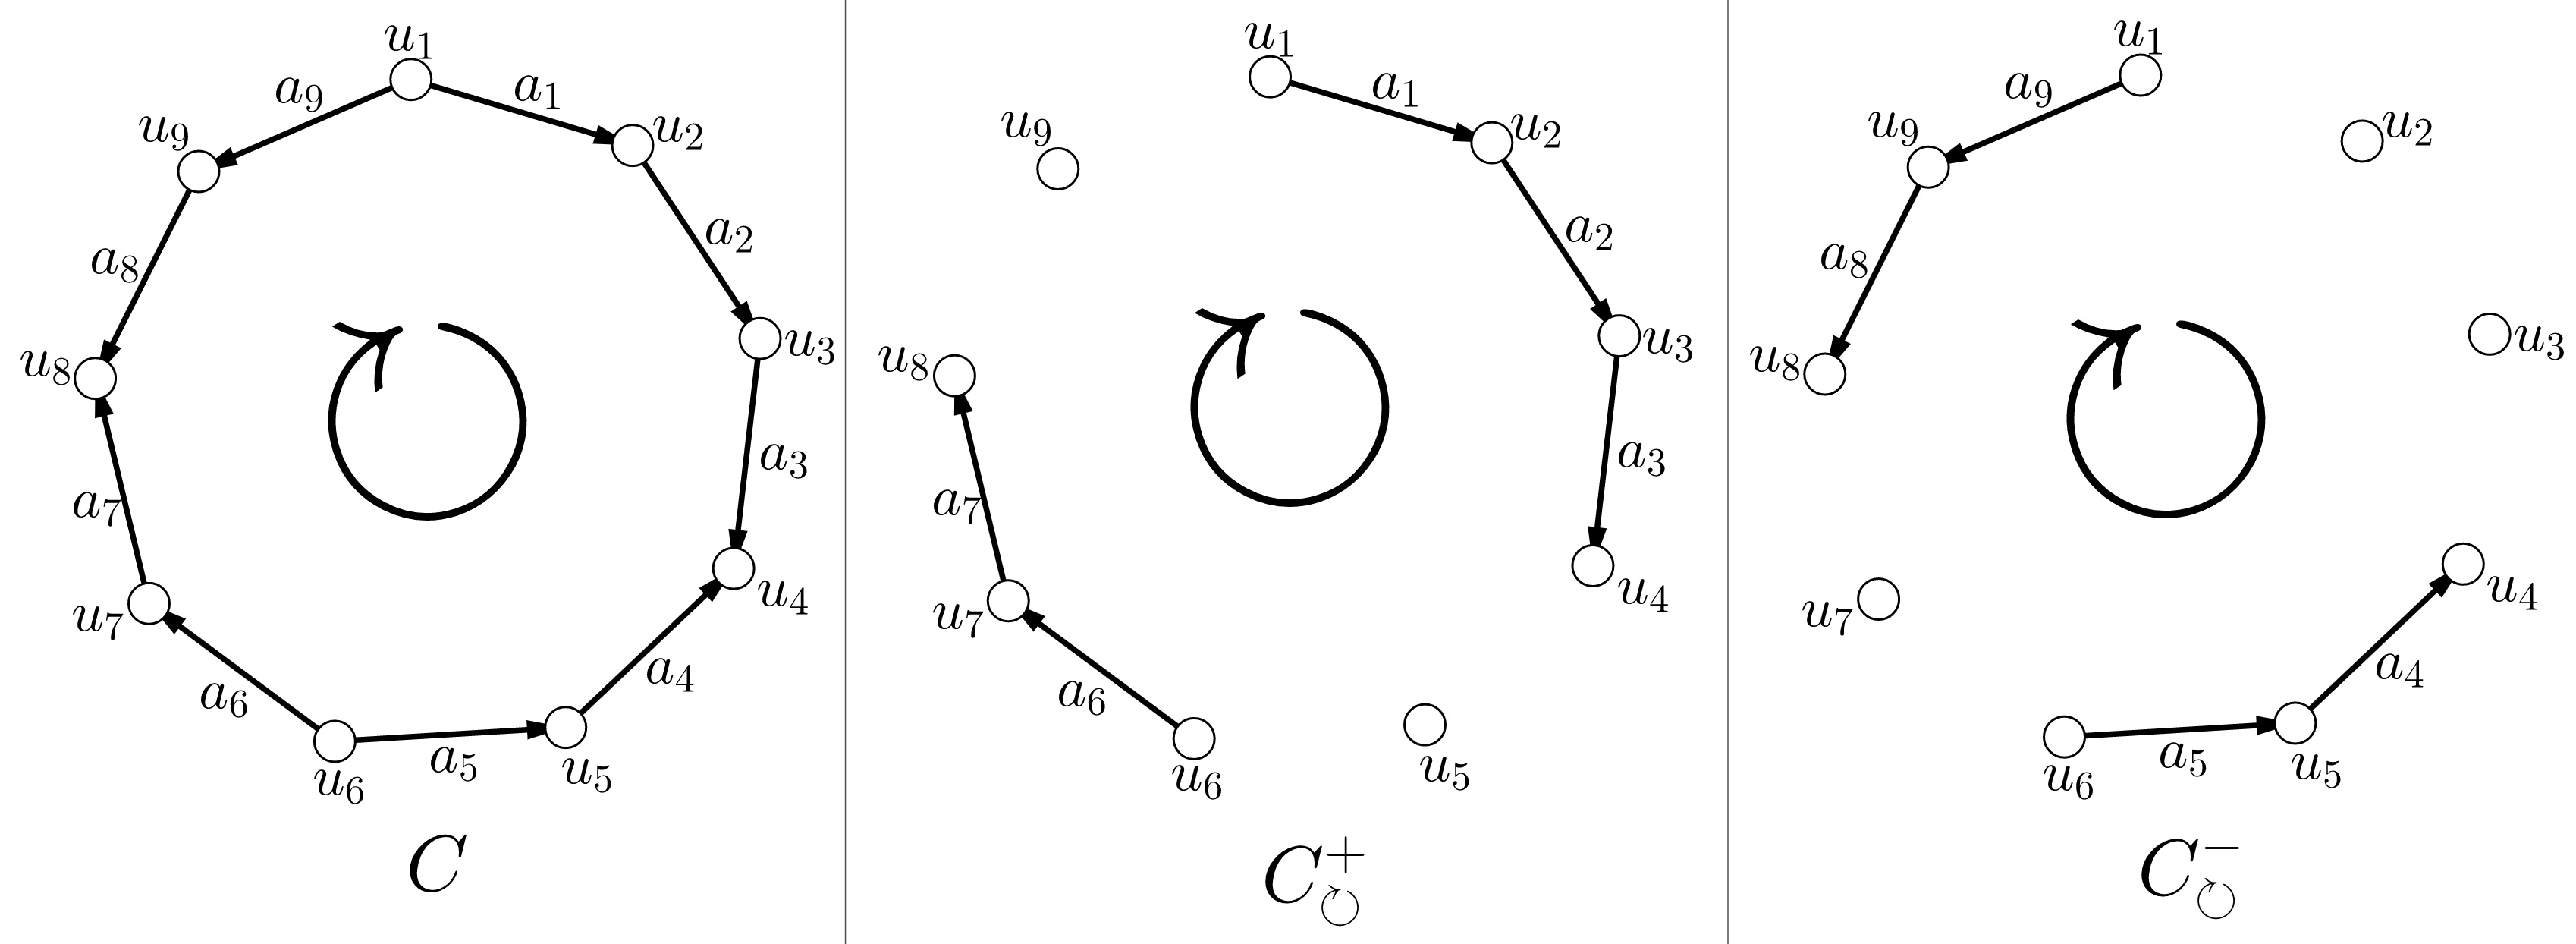
\includegraphics[scale=0.15]{img/imgchapter1/sentidociclos.jpg}
    \caption{}
    \label{fig:ciclosentidos}
\end{figure}

Los conjunto de arcos hacia adelante y hacia atrás de $\Gamma_{\mathbf{\circlearrowright}}$ inducen dos subdigráficas del ciclo $C$, denotados, respectivamente, por $C^{+}_{\mathbf{\circlearrowright}}$ y $C^{-}_{\mathbf{\circlearrowright}}$. De manera similar, $\Gamma_{\mathbf{\circlearrowleft}}$ induce $C^{+}_{\mathbf{\circlearrowleft}}$ y $C^{-}_{\mathbf{\circlearrowleft}}$. Puede verificarse que $C^{+}_{\mathbf{\circlearrowright}}=C^{-}_{\mathbf{\circlearrowleft}}$ y $C^{-}_{\mathbf{\circlearrowright}} = C^{+}_{\mathbf{\circlearrowleft}} $

Sea cual sea el sentido que escojamos, es evidente que $C = C^{+} \cup C^{-}$. Aún más, si para algún sentido se tiene que $C=C^{+}$, entonces $C$ es un \textit{ciclo dirigido}. En la imagen \ref{fig:ciclosentidos} mostramos un ciclo de nueve vértices y, para representar el sentido escogido, dentro de él colocamos el símbolo $\mathbf{\circlearrowright}$. Asimismo, resaltamos los arcos hacia adelante $C^{+}_{\mathbf{\circlearrowright}}$ y los arcos hacia atrás $C^{-}_{\mathbf{\circlearrowright}}$. 


\begin{wrapfigure}{r}{0.3\textwidth}
\vspace{-0.5 cm}
 \centering
  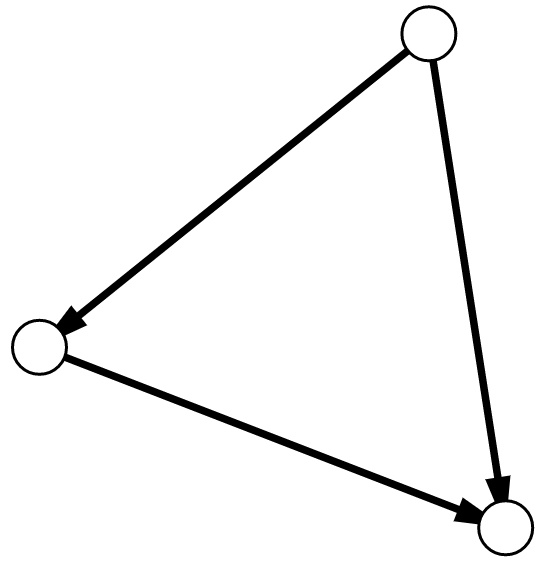
\includegraphics[scale=0.22]{img/imgchapter1/digrafoaciclico.jpg}
  \caption{}
  \label{fig:digrafoaciclico}
  %\vspace{-2 cm}
\end{wrapfigure}

Por último, comentamos que una digráfica se dice que es \textit{acíclica} si no contiene ciclos dirigidos. Por ejemplo, la gráfica de la figura \ref{fig:digrafoaciclico} es acíclica pues, aunque ella misma sea un ciclo, no es un ciclo dirigido. De hecho, se sabe que \textit{toda digráfica acíclica tiene, al menos, una fuente y un pozo.}